\documentclass[a4paper]{report}
\usepackage[utf8]{inputenc}
\usepackage[T1]{fontenc}
\usepackage{RJournal}
\usepackage{amsmath, amssymb, array}
\usepackage{booktabs}
\long\def\comment#1{}    % use \comment{  }  instead of %
\newcommand{\centerfig}[2]{\centerline{\dofig{#1}{#2}}}
\newcommand{\dofig}[2]{\resizebox{#1}{!}{\includegraphics{#2}}}

%% load any required packages here

\begin{document}

%% do not edit, for illustration only
\sectionhead{Contributed research article}
\volume{14}
\volnumber{1}
\year{2022}
\month{March}
\setcounter{page}{167}

%% replace RJtemplate with your article
\begin{article}
  %\begin{document}

\title{\pkg{spherepc}: An R Package for Dimension Reduction on a Sphere}
\author{by Jongmin Lee, Jang-Hyun Kim and Hee-Seok Oh}

\maketitle

\abstract{ 
Dimension reduction is a technique that can compress given data and reduce noise. Recently, a dimension reduction technique on spheres, called spherical principal curves (SPC), has been proposed. SPC fits a curve that passes through the middle of data with a stationary property on spheres. In addition, a study of local principal geodesics (LPG) is considered to identify the complex structure of data. Through the description and implementation of various examples, this paper introduces an R package \CRANpkg{spherepc} for dimension reduction of data lying on a sphere, including existing methods, SPC and LPG.
}


\section{Introduction}
This paper aims to introduce an R package \CRANpkg{spherepc} that considers several dimension reduction techniques on a sphere, which encompass recently developed approaches such as SPC and LPG as well as some existing methods, and discuss  how to implement these methods through \CRANpkg{spherepc}.  

Dimension reduction methods are widely used in various fields, including statistics and machine learning, by efficiently compressing data and removing noise \citep{Benner2005}. As one of the dimension reduction methods, the principal curves of \citet{Hastie1989} are suitable for fitting a curve or a surface of data in Euclidean space, which go through the middle of the data. \citet{Hauberg2016} proposed an algorithm to find the principal curves in Riemannian manifolds based on the concept of the original principal curves. However, the principal curves proposed by \citet{Hauberg2016} no longer represent the data continuously because of the approximation of the projection step required to fit the curves. 

Recently, \citet{Lee2021} proposed a new method, termed spherical principal curves (SPC), that constructs principal curves, ensuring a stationary property on spheres. SPC is useful for representing circular or waveform data with smaller reconstruction errors than conventional methods, including principal geodesic analysis \citep{Fletcher2004}, exact principal circle \citep{Lee2021}, and principal curves proposed by \citet{Hauberg2016}. However, SPC has the disadvantage of being sensitive to initialization. As a result, there are some data structures that SPC does not apply to, for example, data with spirals, zigzags, or branches like tree-shape. A localized version of SPC called local principal geodesics (LPG) is being developed to resolve such a problem. A function for LPG is also provided in the package \CRANpkg{spherepc}. Research on the LPG is underway in progress. 

To the best of our knowledge, no available R packages offer the methods of dimension reduction and principal curves on a sphere. The existing R packages providing principal curves, such as \CRANpkg{princurve} \citep{princurve} and \CRANpkg{LPCM} \citep{LPCM}, are available only on Euclidean space, not on a sphere or (Riemannian) manifold. In addition, most dimension reduction methods on manifolds \citep{Huckemann2010intrinsic, Panaretos2014, Liu2017level} involve somewhat complex optimizations. The proposed package \CRANpkg{spherepc} for R provides the state-of-the-art principal curve technique on the sphere \citep{Lee2021} and comprehensively collects and implements the existing methods \citep{Fletcher2004, Hauberg2016}.

The rest of this paper is organized as follows. The following section introduces the existing methods for dimension reduction on the sphere and relevant functions covered in the package \CRANpkg{spherepc}, which is available on CRAN. Furthermore, their usages are discussed with examples in detail. Then, the spherical principal curves proposed by \cite{Lee2021} and principal curves of \cite{Hauberg2016} are briefly described. In addition, implementations of the \code{SPC()} and \code{SPC.Hauberg()} functions in the \CRANpkg{spherepc} are presented. The subsequent section discusses the local principal geodesics (LPG) with the implementation of various simulated data, demonstrating its promising usability. In the application session, all the mentioned methods are performed to analyze real seismological data. Finally, conclusions are given in the last section. 


\section{Existing methods}\label{sec:method}
\subsection{Principal geodesic analysis}
Principal geodesic analysis (PGA) proposed by \citet{Fletcher2004} can be regarded as a generalization of principal component analysis (PCA) to Riemannian manifolds. In particular, \citet{Fletcher2004} performed dimension reduction of data on the Cartesian product space of the manifolds. In detail, the data are projected onto the tangent spaces at the intrinsic means of each component of the manifolds; thus, the given data are approximated as points on Euclidean vector space, and subsequently, PCA is applied to the points. As a result, the dimension reduction can be performed through the inverse of the tangent projections. 

The principal geodesic analysis can be implemented by the \code{PGA()} function available in the \CRANpkg{spherepc}. The detailed usage of the \code{PGA()} function is described as follows.
\begin{example}
    PGA(data, col1 = "blue", col2 = "red")
\end{example}
Before using the \code{PGA()} function, it requires loading the packages \CRANpkg{rgl} \citep{Adler2020}, \CRANpkg{sphereplot} \citep{Robotham2013}, and \CRANpkg{geosphere} \citep{Hijmans2017}. 
The following codes yield an implementation of the \code{PGA()} function. 

\begin{example} 
   #### for all simulated datasets, longitude and latitude are expressed in degrees
   #### example 1: half-great circle data
   > circle <- GenerateCircle(c(150, 60), radius = pi/2, T = 1000)
   > sigma <- 2                             # noise level
   > half.circle <- circle[circle[, 1] < 0, , drop = FALSE]
   > half.circle <- half.circle + sigma * rnorm(nrow(half.circle))
   > PGA(half.circle)

   #### example 2: S-shaped data
   # the dataset consists of two parts: lon ~ Uniform[0, 20], 
   # lat = sqrt(20 * lon - lon^2) + N(0, sigma^2), 
   # lon ~ Uniform[-20, 0], lat = -sqrt(-20 * lon - lon^2) + N(0, sigma^2)
   > n <- 500              
   > sigma <- 1                             # noise level
   > lon <- 60 * runif(n)  
   > lat <- (60 * lon - lon^2)^(1/2) + sigma * rnorm(n)
   > simul.S1 <- cbind(lon, lat)
   > lon2 <- -60 * runif(n)
   > lat2 <- -(-60 * lon2 - lon2^2)^(1/2) + sigma * rnorm(n)
   > simul.S2 <- cbind(lon2, lat2)
   > simul.S <- rbind(simul.S1, simul.S2)
   > PGA(simul.S)
\end{example}
Because a principal geodesic is always a great circle, the \code{PGA()} function is suitable for identifying the global data trend. The implementations of half-circle and S-shaped data are displayed in Figure~\ref{fig:PGA}, where the principal geodesic properly extracts the global trends in the half-great circle and S-shaped data, while it cannot identify the circular variations in the S-shaped case. In addition, the arguments and outputs of the \code{PGA()} function are described in Tables~\ref{table:PGA} and \ref{table:PGAout}.

\begin{figure}[!h]
    \centering
    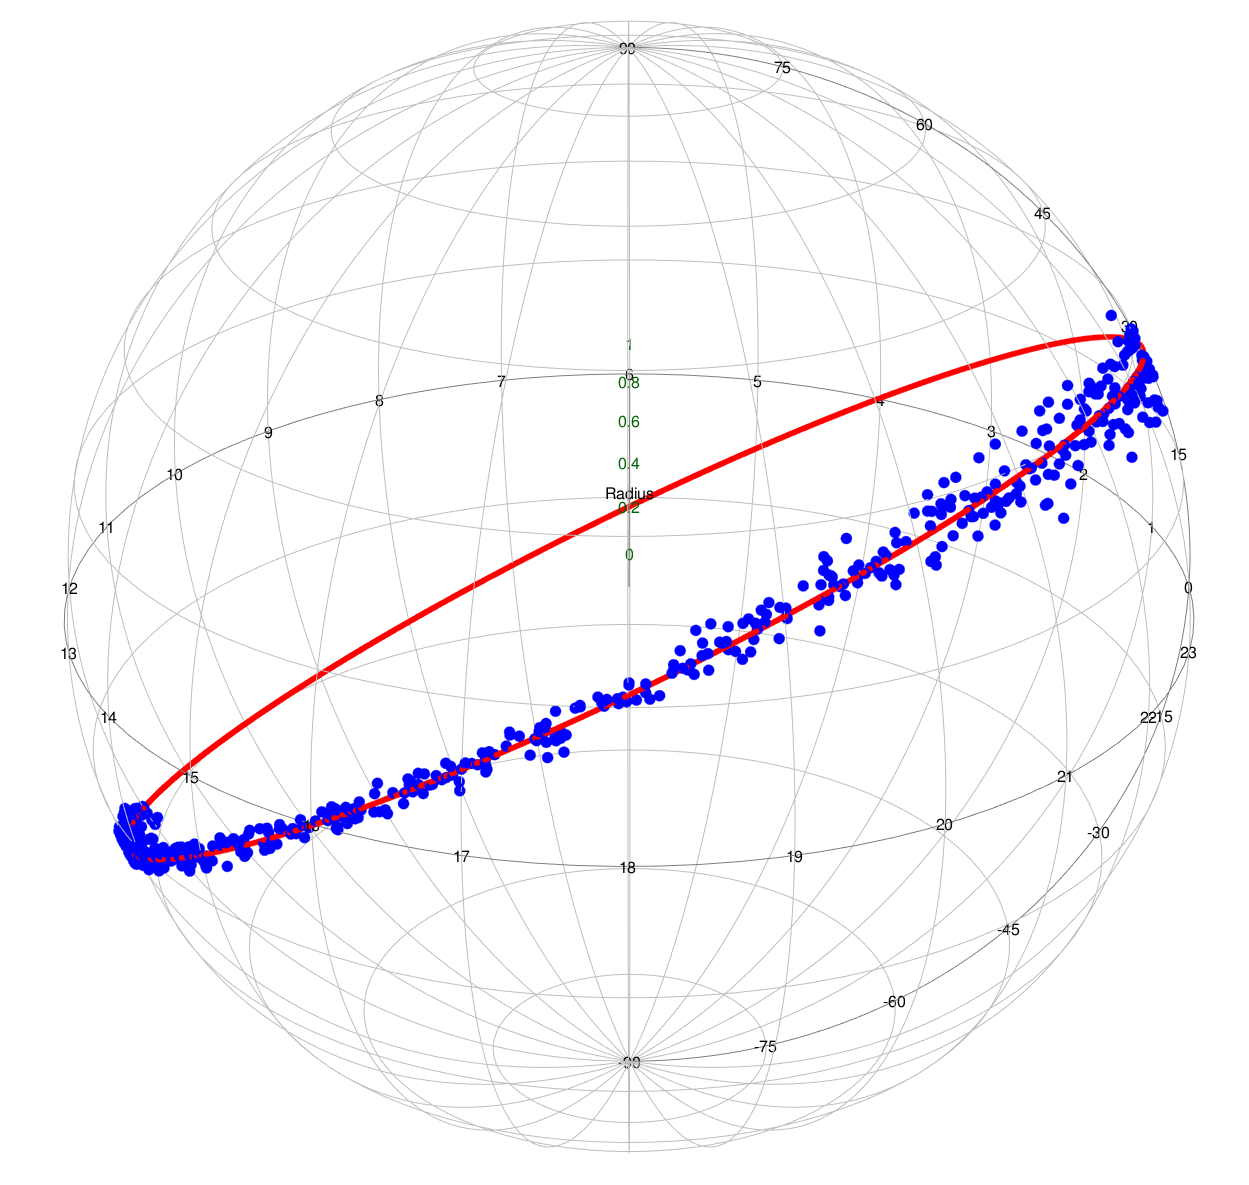
\includegraphics[scale=0.13]{figures/PGA(halfcircle).png}
    \hspace{1cm}
    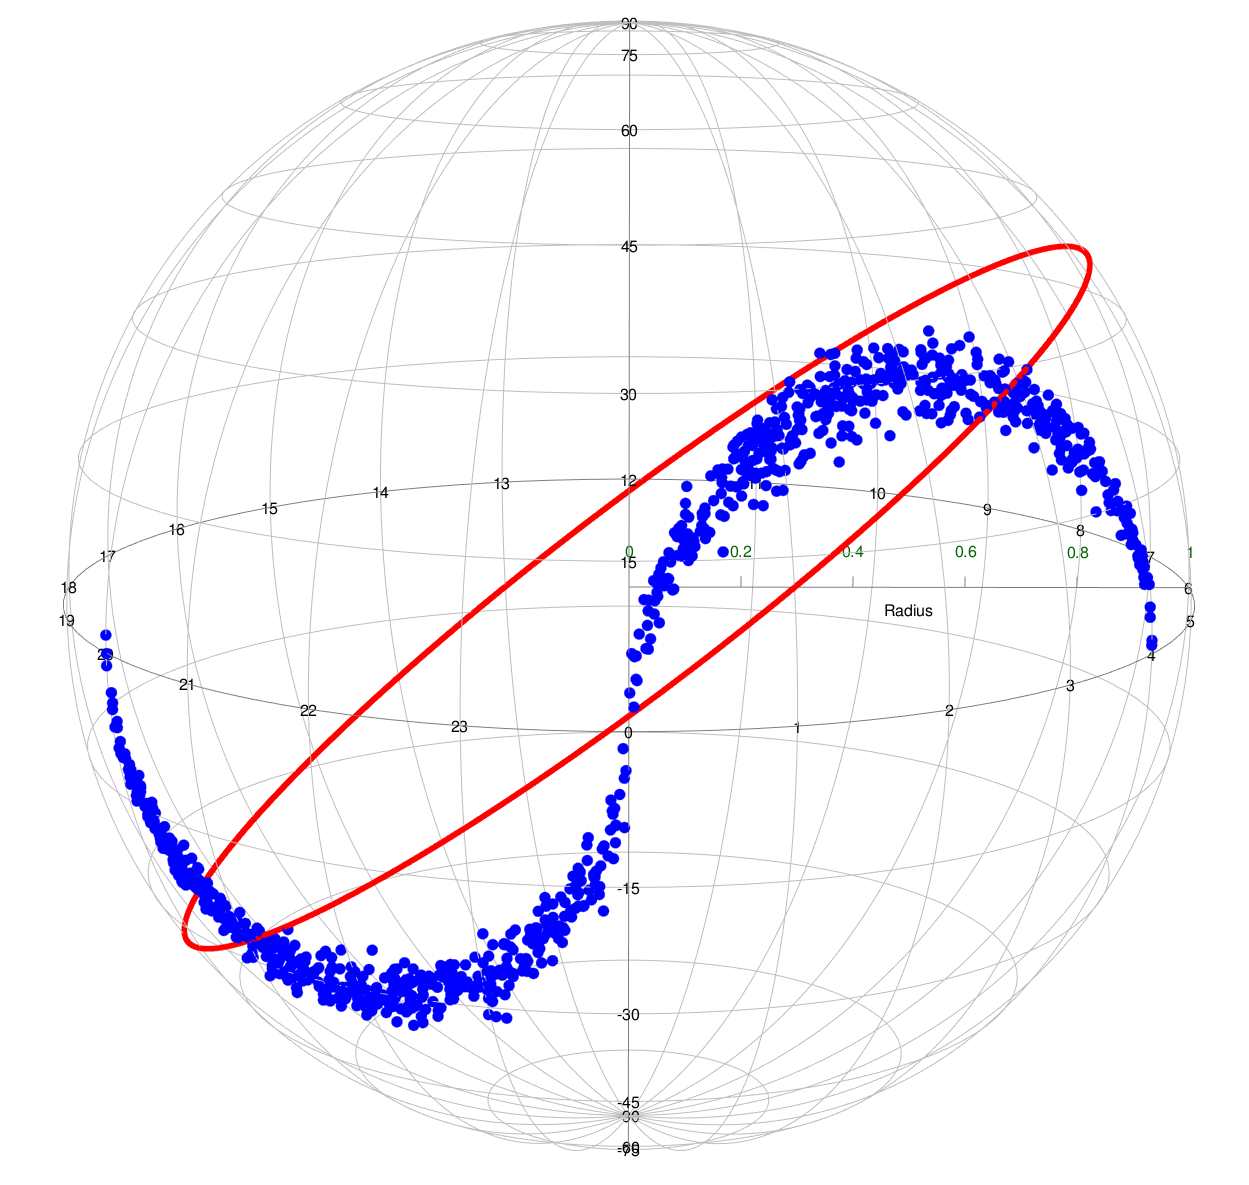
\includegraphics[scale=0.13]{figures/PGA(S).png}
    \caption{From left to right, half-great circle and S-shaped data (blue) and the results (red) of principal geodesic analysis (PGA). The principal geodesic detects the global trends of the noisy half-great circle and the S-shaped data but cannot identify the circular variation of the S-shaped data.}
    \label{fig:PGA}
\end{figure}

\begin{table}[!h]
\centering
\begin{tabular}{lp{0.82 \textwidth}}
\toprule
Argument & Description \\
\midrule	
\code{data} & matrix or data frame consisting of spatial locations with two columns. Each row represents longitude and latitude (denoted by degrees). \\
\code{col1} & color of data. The default is blue. \\
\code{col2} & color of the principal geodesic line. The default is red. \\
\bottomrule
\end{tabular}
\caption{Arguments of the \code{PGA()}.}
\label{table:PGA}
\end{table}


\begin{table}[!h]
\centering
\begin{tabular}{lp{0.82 \textwidth}}
\toprule
Output & Description \\
\midrule
\code{plot} & plotting of the result in 3D graphics. \\
\code{line} & spatial locations (longitude and latitude by degrees) of points in the principal geodesic line. \\
\bottomrule
\end{tabular}
\caption{Outputs of the \code{PGA()}.}
\label{table:PGAout}
\end{table}


\subsection{Principal circle}
In a spherical surface, as shown in Figure~\ref{fig:PGA}, the principal geodesic analysis always results in a great circle, which cannot be sufficient to identify the non-geodesic structure of data. The circle on a sphere that minimizes a reconstruction error is called a principal circle, where the reconstruction error is defined as the total sum of squares of geodesic distances between the circle and data points. However, the existing method for generating the principal circle is still based on the tangent space approximation and its inverse process, thereby leading to numerical errors. \citet{Lee2021} have proposed an exact principal circle in an intrinsic way and its practical algorithm based on gradient descent. The details are described in Section 3 of \citet{Kim2020} and Appendix B of \citet{Lee2021spherical:supp}. The \CRANpkg{spherepc} package provides the \code{PrincipalCircle()} function to implement the intrinsic principal circle. Its usage is followed by
\begin{example}
     PrincipalCircle(data, step.size = 1e-3, thres = 1e-5, maxit = 10000).
\end{example}

\begin{table}[!ht]
\centering
\begin{tabular}{lp{0.82 \textwidth}}
\toprule
Argument & Description \\
\midrule	
\code{data} & matrix or data frame consisting of spatial locations (longitude and latitude denoted by degrees) with two columns. \\
\code{step.size} & step size of gradient descent algorithm. For convergence of the algorithm, \code{step.size} is recommended to be below 0.01. The default is 1e-3.\\
\code{thres} & threshold of the stopping condition. The default is 1e-5. \\
\code{maxit} & maximum number of iterations. The default is 10000. \\
\bottomrule
\end{tabular}
\caption{Arguments of the \code{PrincipalCircle()}.}
\label{table:PrincipalCircle}
\end{table}The arguments of the \code{PrincipalCircle()} are described in Table~\ref{table:PrincipalCircle}, and its output is a three-dimensional vector, where the first and second components are longitude and latitude (represented by degrees), respectively. The last one is the radius of the principal circle. To display the circle, the \code{GenerateCircle()} function should be implemented. Its usage is followed by
\begin{example}
    GenerateCircle(center, radius, T = 1000).
\end{example}
The output of the \code{GenerateCircle()} function is a matrix consisting of spatial locations (longitude and latitude by degrees) with two columns, which can be plotted by the \code{sphereplot::rgl.sphgrid()} and \code{sphereplot::rgl.sphpoints()} functions from the \CRANpkg{sphereplot} package \citep{Robotham2013}. Note that the \CRANpkg{sphereplot} package depends on the \CRANpkg{rgl} package \citep{Adler2020}. The detailed arguments of the \code{GenerateCircle()} function are described in Table~\ref{table:GenerateCircle}.

\begin{table}[!ht]
\centering
\begin{tabular}{lp{0.82 \textwidth}}
\toprule
Argument & Description \\
\midrule	
\code{center} & center of circle with spatial locations (longitude and latitude denoted by degrees). \\
\code{radius} & radius of circle. It should be range from 0 to $\pi$. \\
\code{T} & the number of points that make up a circle. The points in a circle are equally spaced. The default is 1000. \\
\bottomrule
\end{tabular}
\caption{Arguments of the \code{GenerateCircle()}.}
\label{table:GenerateCircle}
\end{table}The following codes implement principal circles by the \code{PrincipalCircle()} and \code{GenerateCircle()} functions.

\begin{example}
   ## for all the following examples, longitude and latitude are denoted by degrees
   #### example 1: half-great circle data
   > circle <- GenerateCircle(c(150, 60), radius = pi/2, T = 1000)
   > half.great.circle <- circle[circle[, 1] < 0, , drop = FALSE]
   > sigma <- 2                           # noise level
   > half.great.circle <- half.great.circle + sigma * rnorm(nrow(half.great.circle))
   ## find a principal circle
   > PC <- PrincipalCircle(half.great.circle)
   > result <- GenerateCircle(PC[1:2], PC[3], T = 1000)
   ## plot the half-great circle data and principal circle
   > sphereplot::rgl.sphgrid(col.lat = "black", col.long = "black")
   > sphereplot::rgl.sphpoints(half.great.circle, radius = 1, col = "blue", size = 9)
   > sphereplot::rgl.sphpoints(result, radius = 1, col = "red", size = 6)

   #### example 2: circular data
   > n <- 700                             # the number of samples
   > sigma <- 5                           # noise level 
   > x <- seq(-180, 180, length.out = n)
   > y <- 45 + sigma * rnorm(n)
   > simul.circle <- cbind(x, y)
   ## find a principal circle
   > PC <- PrincipalCircle(simul.circle)
   > result <- GenerateCircle(PC[1:2], PC[3], T = 1000)
   ## plot the circular data and principal circle
   > sphereplot::rgl.sphgrid(col.lat = "black", col.long = "black")
   > sphereplot::rgl.sphpoints(simul.circle, radius = 1, col = "blue", size = 9)
   > sphereplot::rgl.sphpoints(result, radius = 1, col = "red", size = 6)
\end{example}
The results of the principal circle are shown in Figure~\ref{fig:PC}. As one can see, the principal circle identifies the circular patterns of the noisy half-great circle and circular dataset well.

\begin{figure}[h]
    \centering
    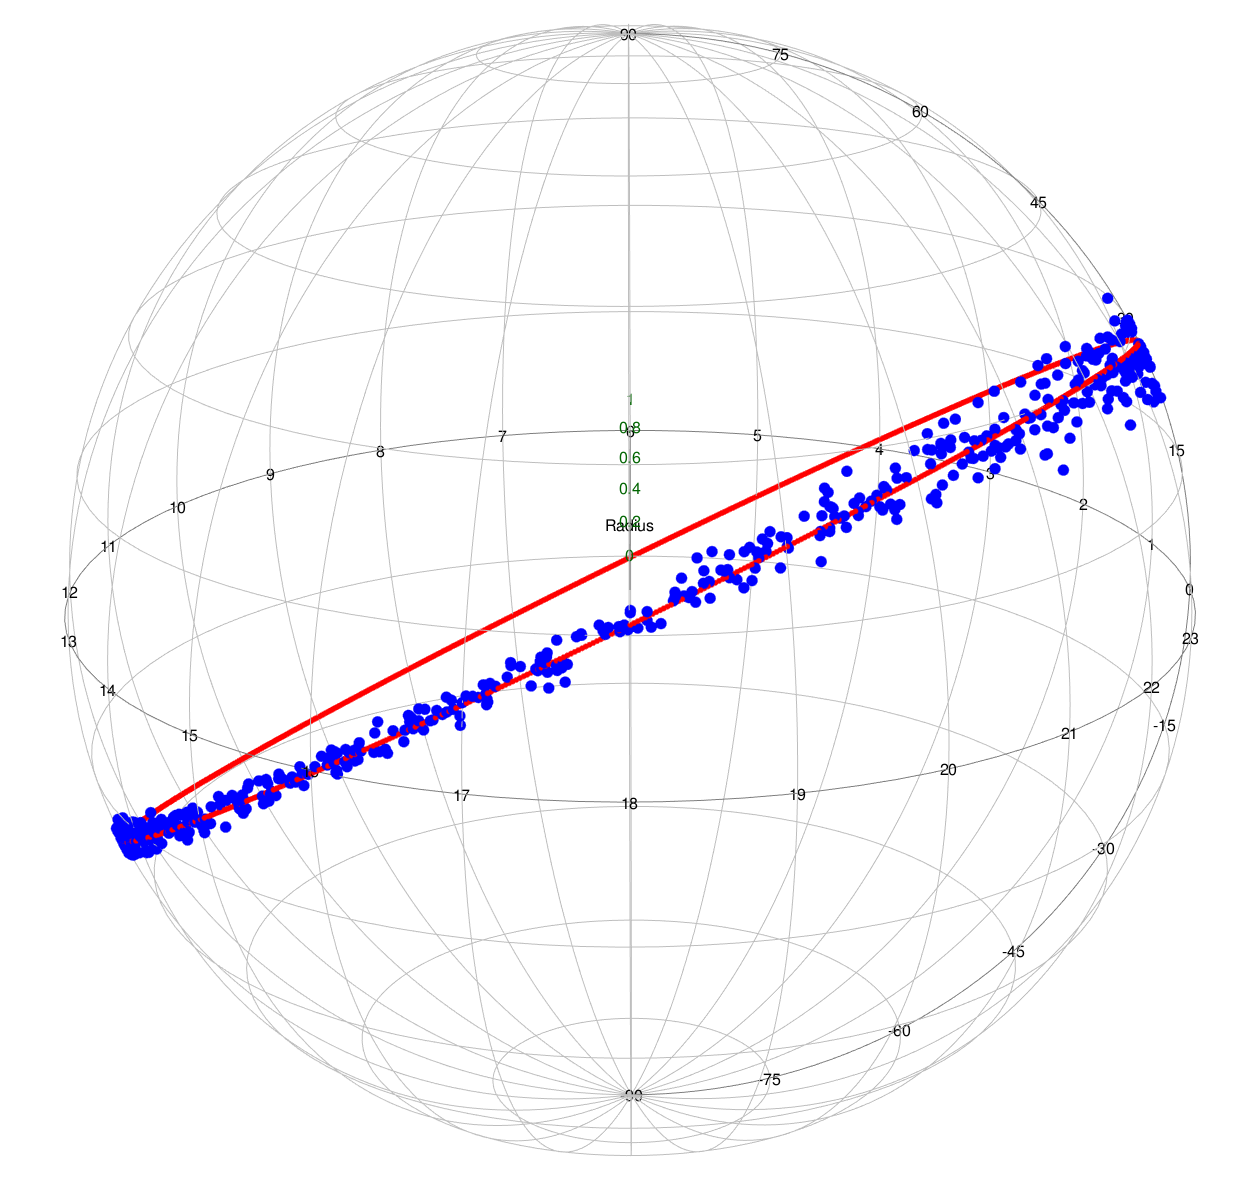
\includegraphics[scale=0.13]{figures/PC(halfcircle).png}
    \hspace{1cm}
    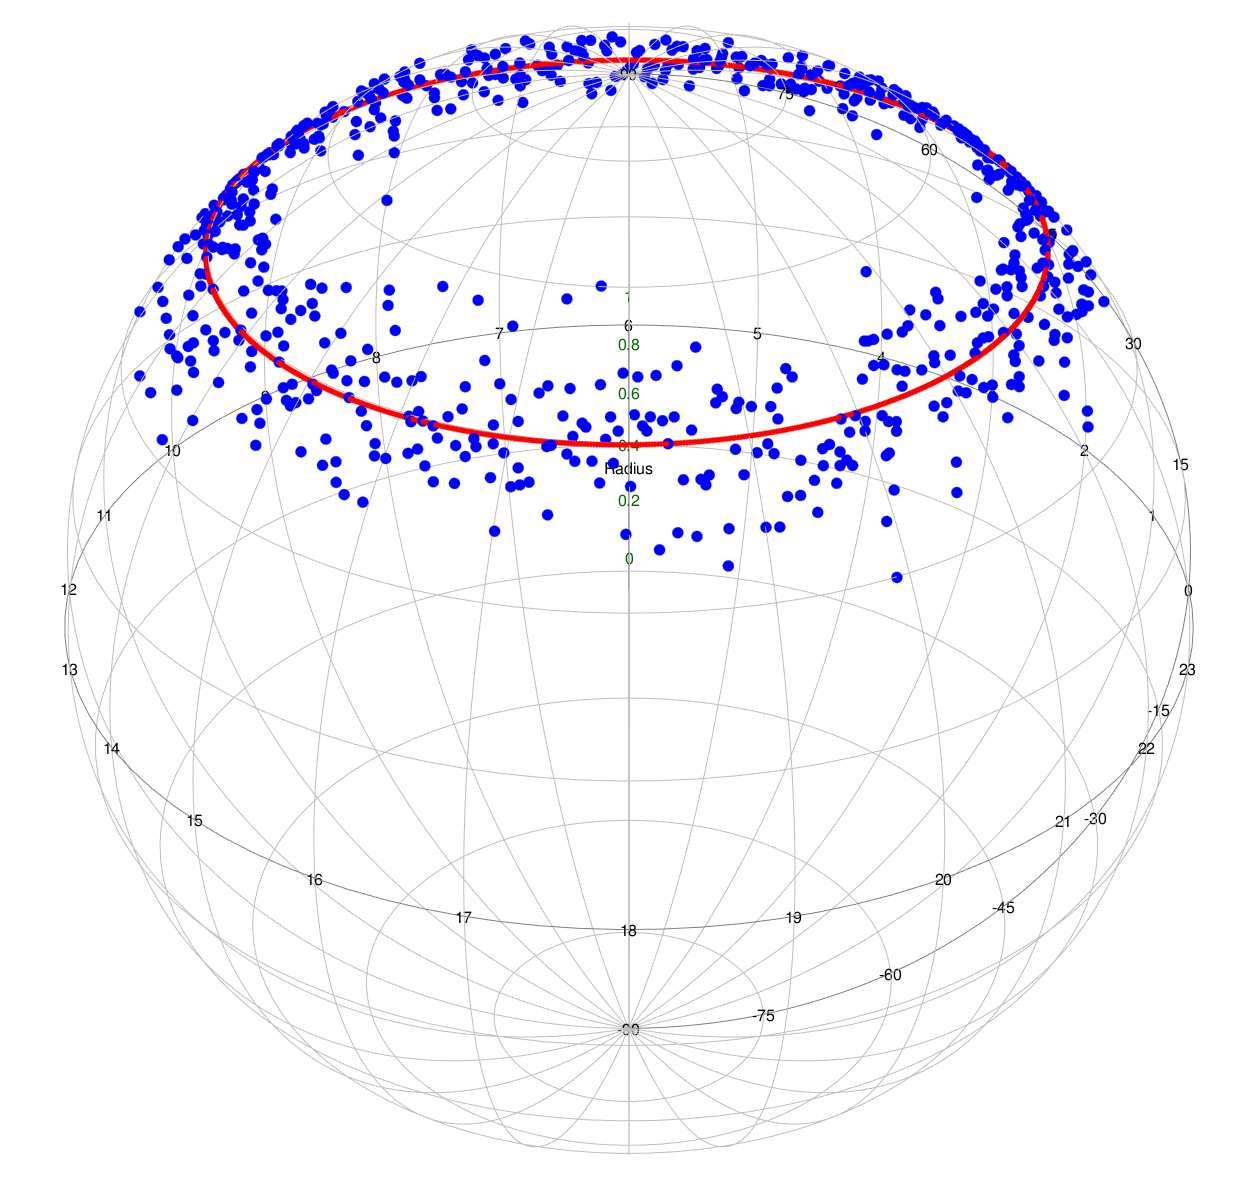
\includegraphics[scale=0.13]{figures/PC(circular).png}
    \caption{Half-great circle data and circular data (blue) and the results (red) of the principal circle from left to right. The principal circle can identify the relatively small circular structure (right) and the great circle structure (left).}
    \label{fig:PC}
\end{figure}


\section{Spherical principal curves}
Principal curves proposed by \citet{Hastie1989} can be considered as a nonlinear generalization of the principal component analysis in the sense that the principal curves pass through the middle of given data and reserve a stationary property. The curve is a smooth function from a one-dimensional closed interval to a given space; then, a curve $f$ is said to be a principal curve of $X$ or self-consistent if the curve satisfies 
\begin{equation*}
f(\lambda) = \mathbb{E}\big(X \ | \ \lambda_{f}(X)=\lambda\big),
\end{equation*}
where $f(\lambda_f(x))$ is the closest (projection) point in the curve $f$ from the point $x$.

\citet{Hauberg2016} provided an algorithm for principal curves on Riemannian manifolds. However, \citet{Hauberg2016} used approximations for finding the closest point of each data point, which may lead to numerical errors. Recently, \citet{Lee2021} presented theoretical results of principal curves on spheres and a practical algorithm for constructing principal curves without any approximations, called spherical principal curves (SPC), thereby causing the given data to be represented more precisely and smoothly compared to principal curves of \citet{Hauberg2016}. In the both ways of extrinsic and intrinsic approaches, the method of SPC updates curves on the spherical surfaces to represent the given data and fits curves that satisfy the stationary conditions. For more details, refer to \citet{Kim2020} or \citet{Lee2021}.

The package \CRANpkg{spherepc} provides the \code{SPC()} function for implementing spherical principal curves and the \code{SPC.Hauberg()} function for principal curves of \citet{Hauberg2016}. The usage of the \code{SPC()} function is as follows.
\begin{example}
    SPC(data, q = 0.05, T = nrow(data), step.size = 1e-3, maxit = 30,
        type = "Intrinsic", thres = 1e-2, deletePoints = FALSE,  
        plot.proj = FALSE, kernel = "quartic", col1 = "blue", 
        col2 = "green", col3 = "red").
\end{example}
The usage of the \code{SPC.Hauberg()} function is the same as that of the \code{SPC()} function. Before implementing the \code{SPC()} and \code{SPC.Hauberg()} functions, it requires loading the \CRANpkg{rgl} \citep{Adler2020}, \CRANpkg{sphereplot} \citep{Robotham2013}, and \CRANpkg{geosphere} \citep{Hijmans2017} packages. To implement the \code{SPC()} and \code{SPC.Hauberg()} functions, we consider the waveform data used in \citet{Liu2017level}, \citet{Kim2020}, and \citet{Lee2021}. The generating equation of waveform is
\begin{equation*}
    \phi = \alpha\cdot \sin(f \theta\cdot \pi/180) + 10,
\end{equation*}
where $\phi$, $\theta$, $\alpha$, and $f$ denote the longitude, latitude in degrees, amplitude and frequency of the waveform, respectively. $\theta$ is uniformly sampled from the interval $[-180,\, 180]$ and a Gaussian random noise from $N(0,\, \sigma^2)$ is added on each $\phi$ where $\sigma = 2,\, 10$. The generating waveform data and implementations of the \code{SPC()} and \code{SPC.Hauberg()} functions are as follows. 
\begin{example}
   #### longitude and latitude are expressed in degrees
   #### example: waveform data
   > n <- 200
   > alpha <- 1/3; freq <- 4                    # amplitude and frequency of wave
   > sigma1 <- 2; sigma2 <- 10                  # noise levels  
   > lon <- seq(-180, 180, length.out = n)      # uniformly sampled longitude
   > lat <- alpha * 180/pi * sin(freq * lon * pi/180) + 10      # latitude vector
   ## add Gaussian noises on the latitude vector
   > lat1 <- lat + sigma1 * rnorm(length(lon))
   > lat2 <- lat + sigma2 * rnorm(length(lon))
   > wave1 <- cbind(lon, lat1); wave2 <- cbind(lon, lat2)
   ## implement Hauberg's principal curves to the waveform data
   > SPC.Hauberg(wave1, q = 0.05)
   ## implement SPC to the (noisy) waveform data
   > SPC(wave1, q = 0.05)
   > SPC(wave2, q = 0.05)
\end{example}
The above codes generate the results in Figure~\ref{SPC:wave}. As one can see, the \code{SPC()} and \code{SPC.Hauberg()} functions identify the waveform pattern of the simulated data. Especially, the \code{SPC()} generates a smoother curve. The detailed arguments and outputs of the \code{SPC()} are described in Tables~ \ref{table:SPC} and \ref{table:SPCout}, respectively, which are the same for the \code{SPC.Hauberg()}.

\begin{figure}[h]
    \centering
    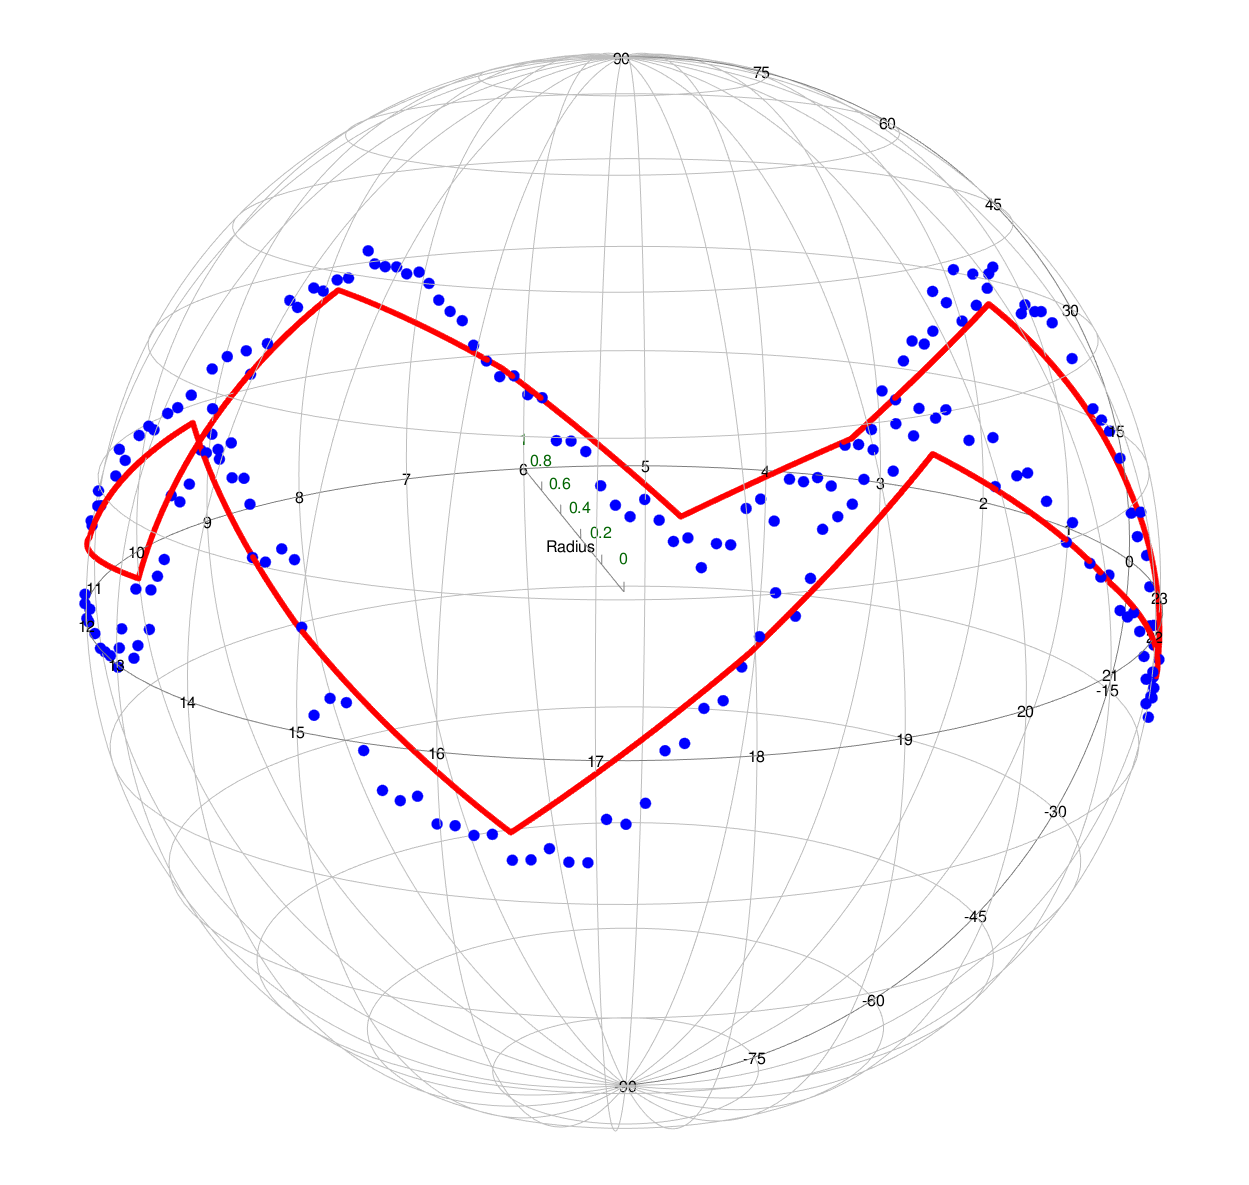
\includegraphics[scale=0.10]{figures/Hauberg(wave).png}
    \hspace{0cm}
    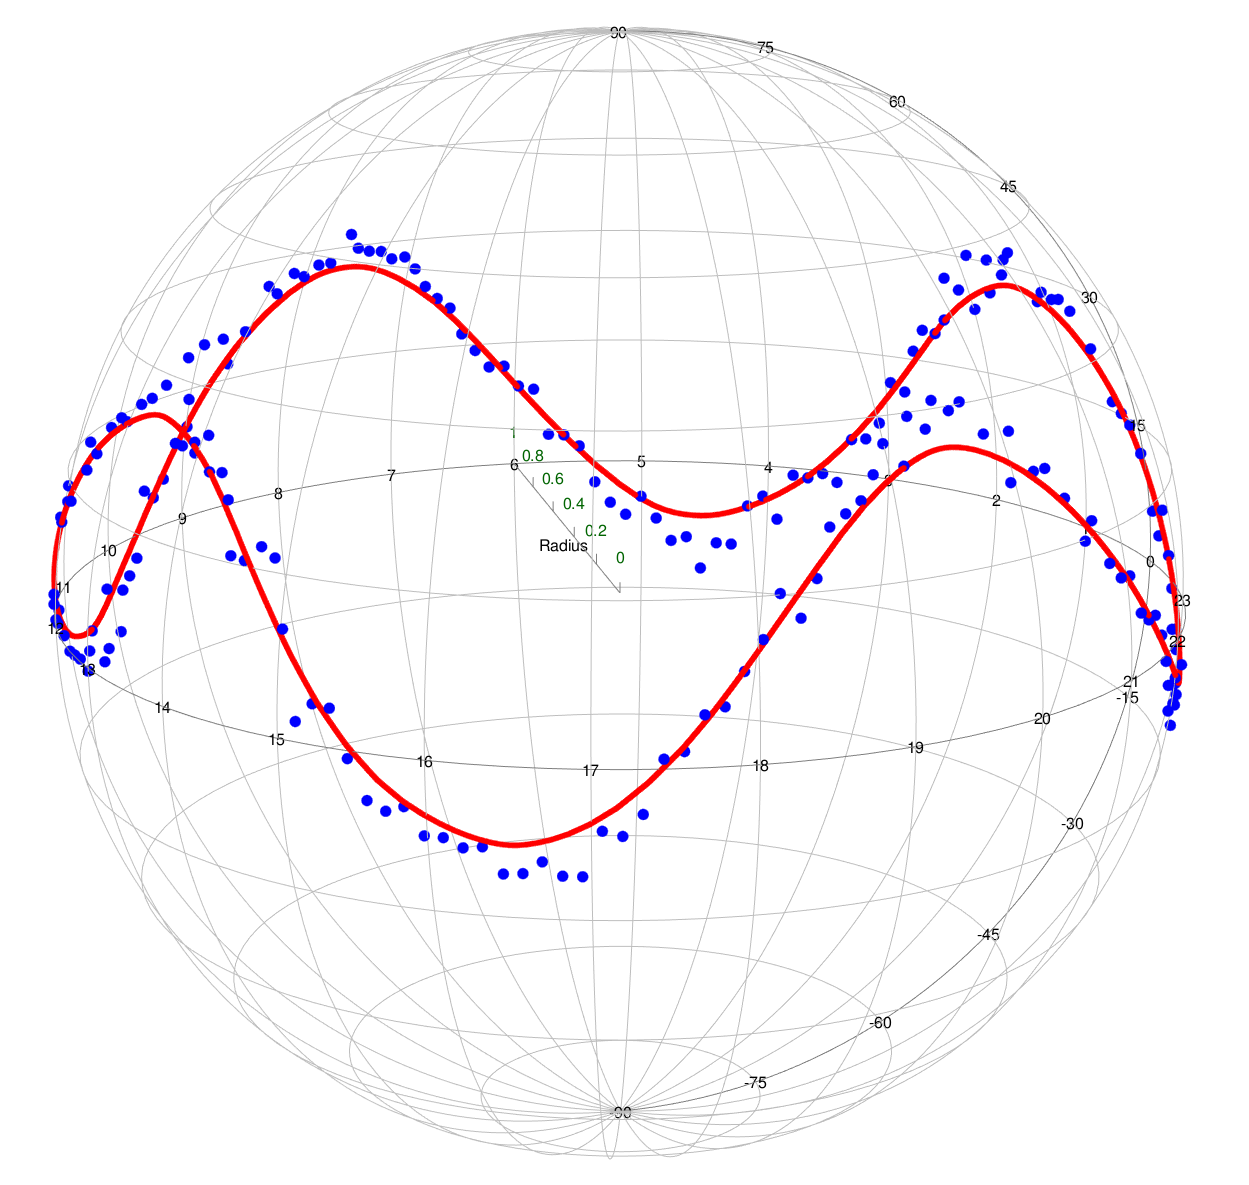
\includegraphics[scale=0.10]{figures/SPC(wave).png}
    \hspace{0.2cm}
    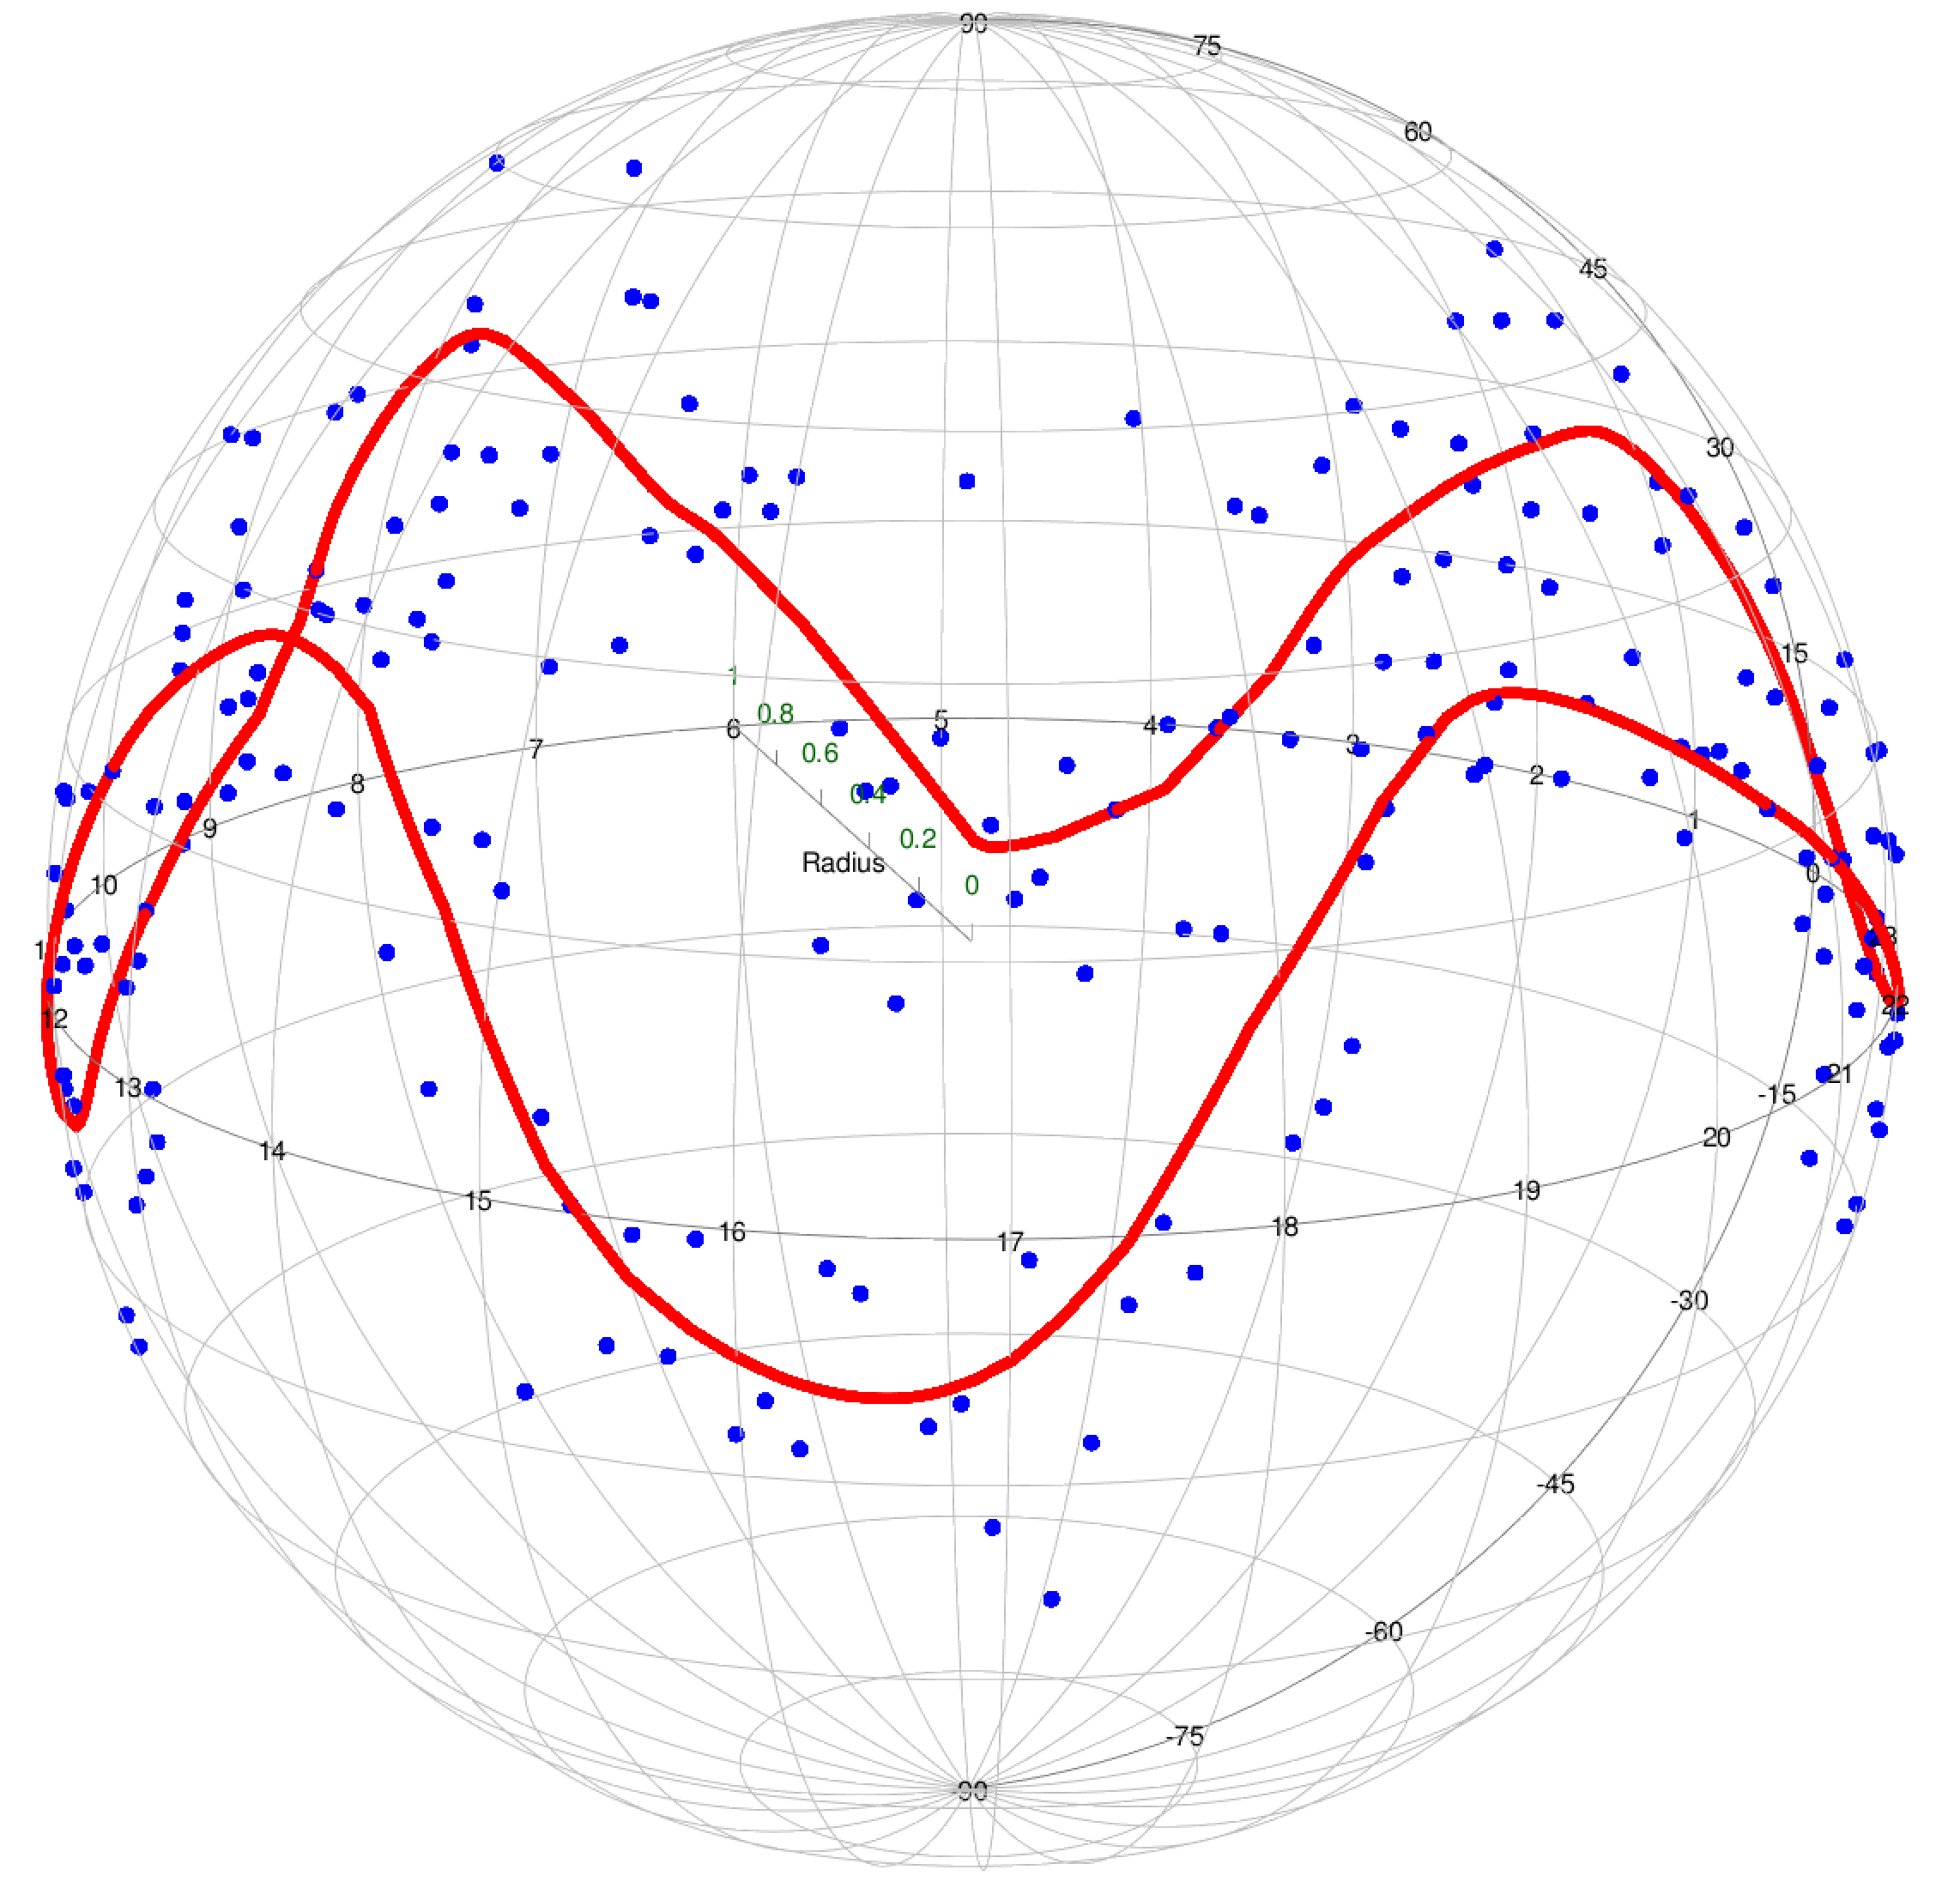
\includegraphics[scale=0.105]{figures/SPC(wave_noisy).png}
    \caption{Left and middle: The waveform data (blue) and the results (red) of Hauberg's principal curves (left) and spherical principal curves. Right: The noisy waveform data (blue) and the result (red) of spherical principal curves. All cases are implemented with $q = 0.05$. The two methods find the true waveform of the data well. In particular, the spherical principal curve tends to be smoother.}
    \label{SPC:wave}
\end{figure}


\begin{table}[!ht]
\centering
\begin{tabular}{lp{0.82 \textwidth}}
\toprule
Argument & Description \\
\midrule	
\code{data} & matrix or data frame consisting of spatial locations with two columns. Each row represents longitude and latitude (denoted by degrees). \\
\code{q} & numeric value of the smoothing parameter. The parameter plays the same role, as the bandwidth does in kernel regression, in the \code{SPC} function. The value should be a numeric value between 0.01 and 0.5. The default is 0.1. \\
\code{T} & the number of points making up the resulting curve. The default is 1000. \\
\code{step.size} & step size of the \code{PrincipalCircle} function. The default is 0.001. The resulting principal circle is used as an initialization of the \code{SPC} function. \\
\code{maxit} & maximum number of iterations. The default is 30. \\
\code{type} & type of mean on the sphere. The default is "Intrinsic" and the other choice is "Extrinsic". \\
\code{thres} & threshold of the stopping condition. The default is 0.01. \\
\code{deletePoints} & logical value. The argument is an option of whether to delete points or not. If \code{deletePoints} is FALSE, this function leaves the points in curves that do not have adjacent data for each expectation step. As a result, the function usually returns a closed curve, \textit{i.e.} a curve without endpoints. If \code{deletePoints} is TRUE, this function deletes the points in curves that do not have adjacent data for each expectation step. As a result, The \code{SPC} function usually returns an open curve, \textit{i.e.} a curve with endpoints. The default is FALSE. \\
\code{plot.proj} & logical value. If the argument is TRUE, the projection line for each data point is plotted. The default is FALSE. \\ 
\code{kernel} & kind of kernel function. The default is the quartic kernel, and the alternative is indicator or Gaussian. \\
\code{col1} & color of data. The default is blue.\\
\code{col2} & color of points in principal curves. The default is green. \\
\code{col3} & color of resulting principal curves. The default is red.\\
\bottomrule
\end{tabular}
\caption{Arguments of the \code{SPC()}.}
\label{table:SPC}
\end{table}

\begin{table}[!ht]
\centering
\begin{tabular}{lp{0.82 \textwidth}}
\toprule
Output & Description \\
\midrule
\code{plot} & plotting of the result in 3D graphics. \\
\code{prin.curves} & spatial locations (denoted by degrees) of points in the resulting principal curves.\\
\code{line} & connecting lines between points in \code{prin.curves}. \\
\code{converged} & whether or not the algorithm converged. \\
\code{iteration} & the number of iterations of the algorithm. \\
\code{recon.error} & sum of squared distances between the data and their projections. \\
\code{num.dist.pt} & the number of distinct projections. \\
\bottomrule
\end{tabular}
\caption{Outputs of the \code{SPC()}.}
\label{table:SPCout}
\end{table}

\subsection{Options for spherical principal curves}
There are some options for the \code{SPC()} and \code{SPC.Hauberg()} functions. In particular, we implement using the arguments \code{plot.proj} and \code{deletePoints}, described in Table~\ref{table:SPC}. If \code{plot.proj = TRUE} is used, then the projection line for each data point is plotted. If the argument \code{deletePoints = TRUE} is performed, the \code{SPC()} function deletes the points in curves that do not have adjacent data for each expectation step required to fit the principal curves, returning an open curve, \textit{i.e.}, a curve with endpoints. As a result, the principal curves are more parsimonious since a redundant part of the resulting curves is removed. The \code{SPC.Hauberg()} function also contains the same options. For implementing these two arguments, the following codes are performed through real earthquake data.

\begin{example}
   > data(Earthquake)
   # collect spatial locations (longitude and latitude denoted by degrees) of data
   > earthquake <- cbind(Earthquake$longitude, Earthquake$latitude)
   
   #### example 1: plot the projection lines (option of plot.proj)
   > SPC(earthquake, q = 0.1, plot.proj = TRUE)

   #### example 2: open principal curves (option of deletePoints)
   > SPC(earthquake, q = 0.04, deletePoints = TRUE)
\end{example}
The results are illustrated in Figure~\ref{fig:SPCoption}. The left panel shows a closed principal curve (red) with projection lines (black) of each data point onto the curve, and the right panel displays an open principal curve due to the option \code{deletePoints = TRUE}. It is a parsimonious result because the redundant part on the upper right side of the sphere is removed.

\begin{figure}[h]
    \centering
    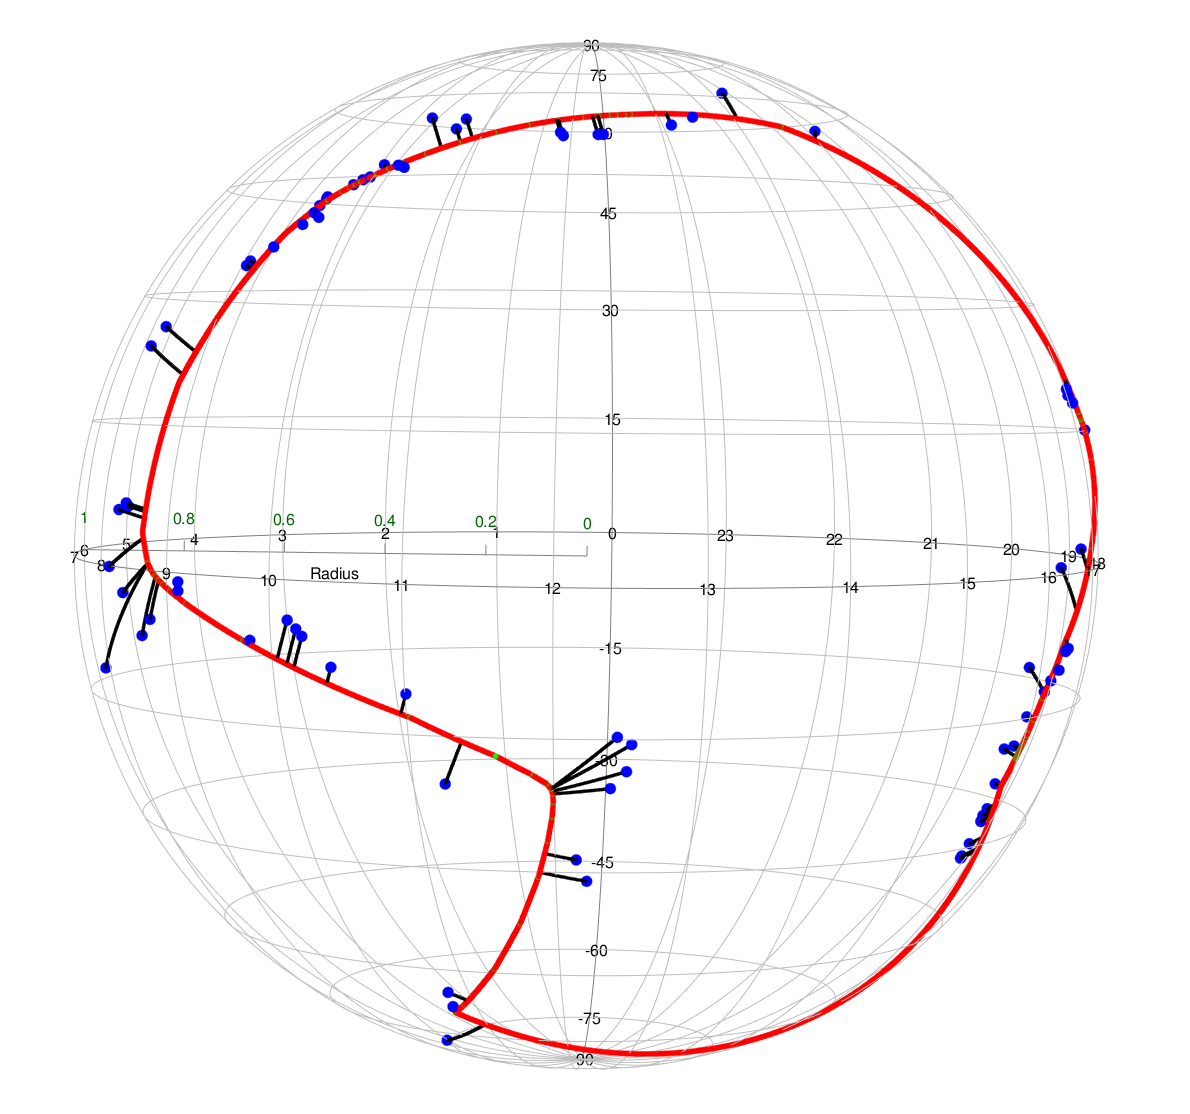
\includegraphics[scale=0.147]{{figures/SPC(option1).png}}
    \hspace{0.3cm}
    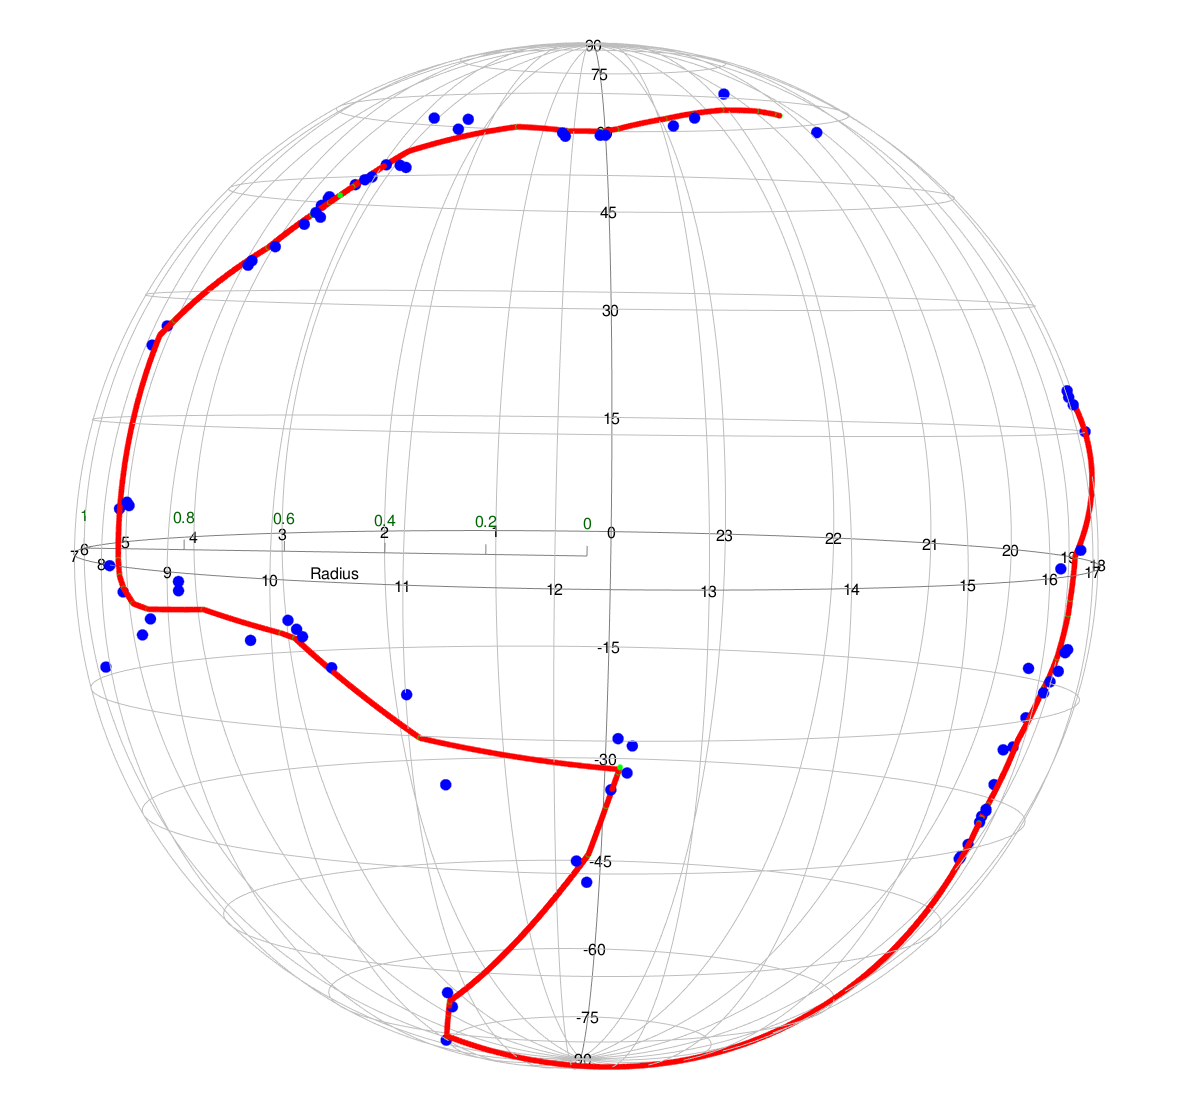
\includegraphics[scale=0.147]{{figures/SPC(option2).png}}
    \caption{Left: Projection result (black) of SPC with $q = 0.1$. The spherical principal curve (red) continuously represents the earthquake data (blue). Right: The open curve of SPC with $q = 0.04$ and \code{deletePoints=TRUE}. The less $q$ is, the more the curve overfits the data.}
    \label{fig:SPCoption}
\end{figure}

\section{Local principal geodesics}\label{lpg}
Suppose that observations have a non-geodesic structure. Then the PGA may not be beneficial to represent such data because PGA always results in a geodesic line. To overcome this problem, we consider performing PGA locally and repeatedly to detect the non-geodesic and complex structures of data, which can be interpreted as a localized version of the PGA and SPC. The newly proposed method is called local principal geodesics (LPG). The main idea behind the LPG is that non-geodesic structures can be regarded as a part of geodesic when viewed locally. Although there is no reference to the LPG because research on LPG is underway, there is a localized principal curve method on Euclidean space \citep{Einbeck2005local}, which is similar to LPG and may share some motivation with the LPG. For more details, refer to \cite{Einbeck2005local}.

The package \CRANpkg{spherepc} offers the \code{LPG()} function to recognize various data structures, such as spirals, zigzag, and tree data. The usage of the function is
\begin{example}
    LPG(data, scale = 0.04, tau = scale/3, nu = 0, maxpt = 500,
        seed = NULL, kernel = "indicator", thres = 1e-4, col1 = "blue", 
        col2 = "green", col3 = "red").
\end{example}
Like the previous functions, before the \code{LPG()} function is implemented, it requires to load the \CRANpkg{rgl} \citep{Adler2020}, \CRANpkg{sphereplot} \citep{Robotham2013}, and \CRANpkg{geosphere} \citep{Hijmans2017} packages. The detailed arguments and outputs of this function are described in Tables~\ref{table:LPG} and \ref{table:LPGout}. We implement the following code to apply the \code{LPG()} function to the spiral, zigzag, and tree simulated data illustrated in Figures ~\ref{fig:spiral}, \ref{fig:zigzag}, and \ref{fig:tree}.  

\begin{example}
   ## longitude and latitude are expressed in degrees
   #### example 1: spiral data 
   > set.seed(40)
   > n <- 900                                     # the number of samples
   > sigma1 <- 1; sigma2 <- 2.5;                  # noise levels
   > radius <- 73; slope <- pi/16                 # radius and slope of the spiral
   ## polar coordinate of (longitude, latitude)
   > r <- runif(n)^(2/3) * radius; theta <- -slope * r + 3 
   ## transform to (longitude, latitude)
   > correction <- (0.5 * r/radius + 0.3)         # correction of noise level
   > lon1 <- r * cos(theta) + correction * sigma1 * rnorm(n)
   > lat1 <- r * sin(theta) + correction * sigma1 * rnorm(n)
   > lon2 <- r * cos(theta) + correction * sigma2 * rnorm(n)
   > lat2 <- r * sin(theta) + correction * sigma2 * rnorm(n)
   > spiral1 <- cbind(lon1, lat1); spiral2 <- cbind(lon2, lat2)
   ## plot the spiral data
   > rgl.sphgrid(col.lat = 'black', col.long = 'black')
   > rgl.sphpoints(spiral1, radius = 1, col = 'blue', size = 12)
   ## implement the LPG to (noisy) spiral data
   > LPG(spiral1, scale = 0.06, nu = 0.1, seed = 100)
   > LPG(spiral2, scale = 0.12, nu = 0.1, seed = 100)
\end{example}

\begin{figure}[h]
    \centering
    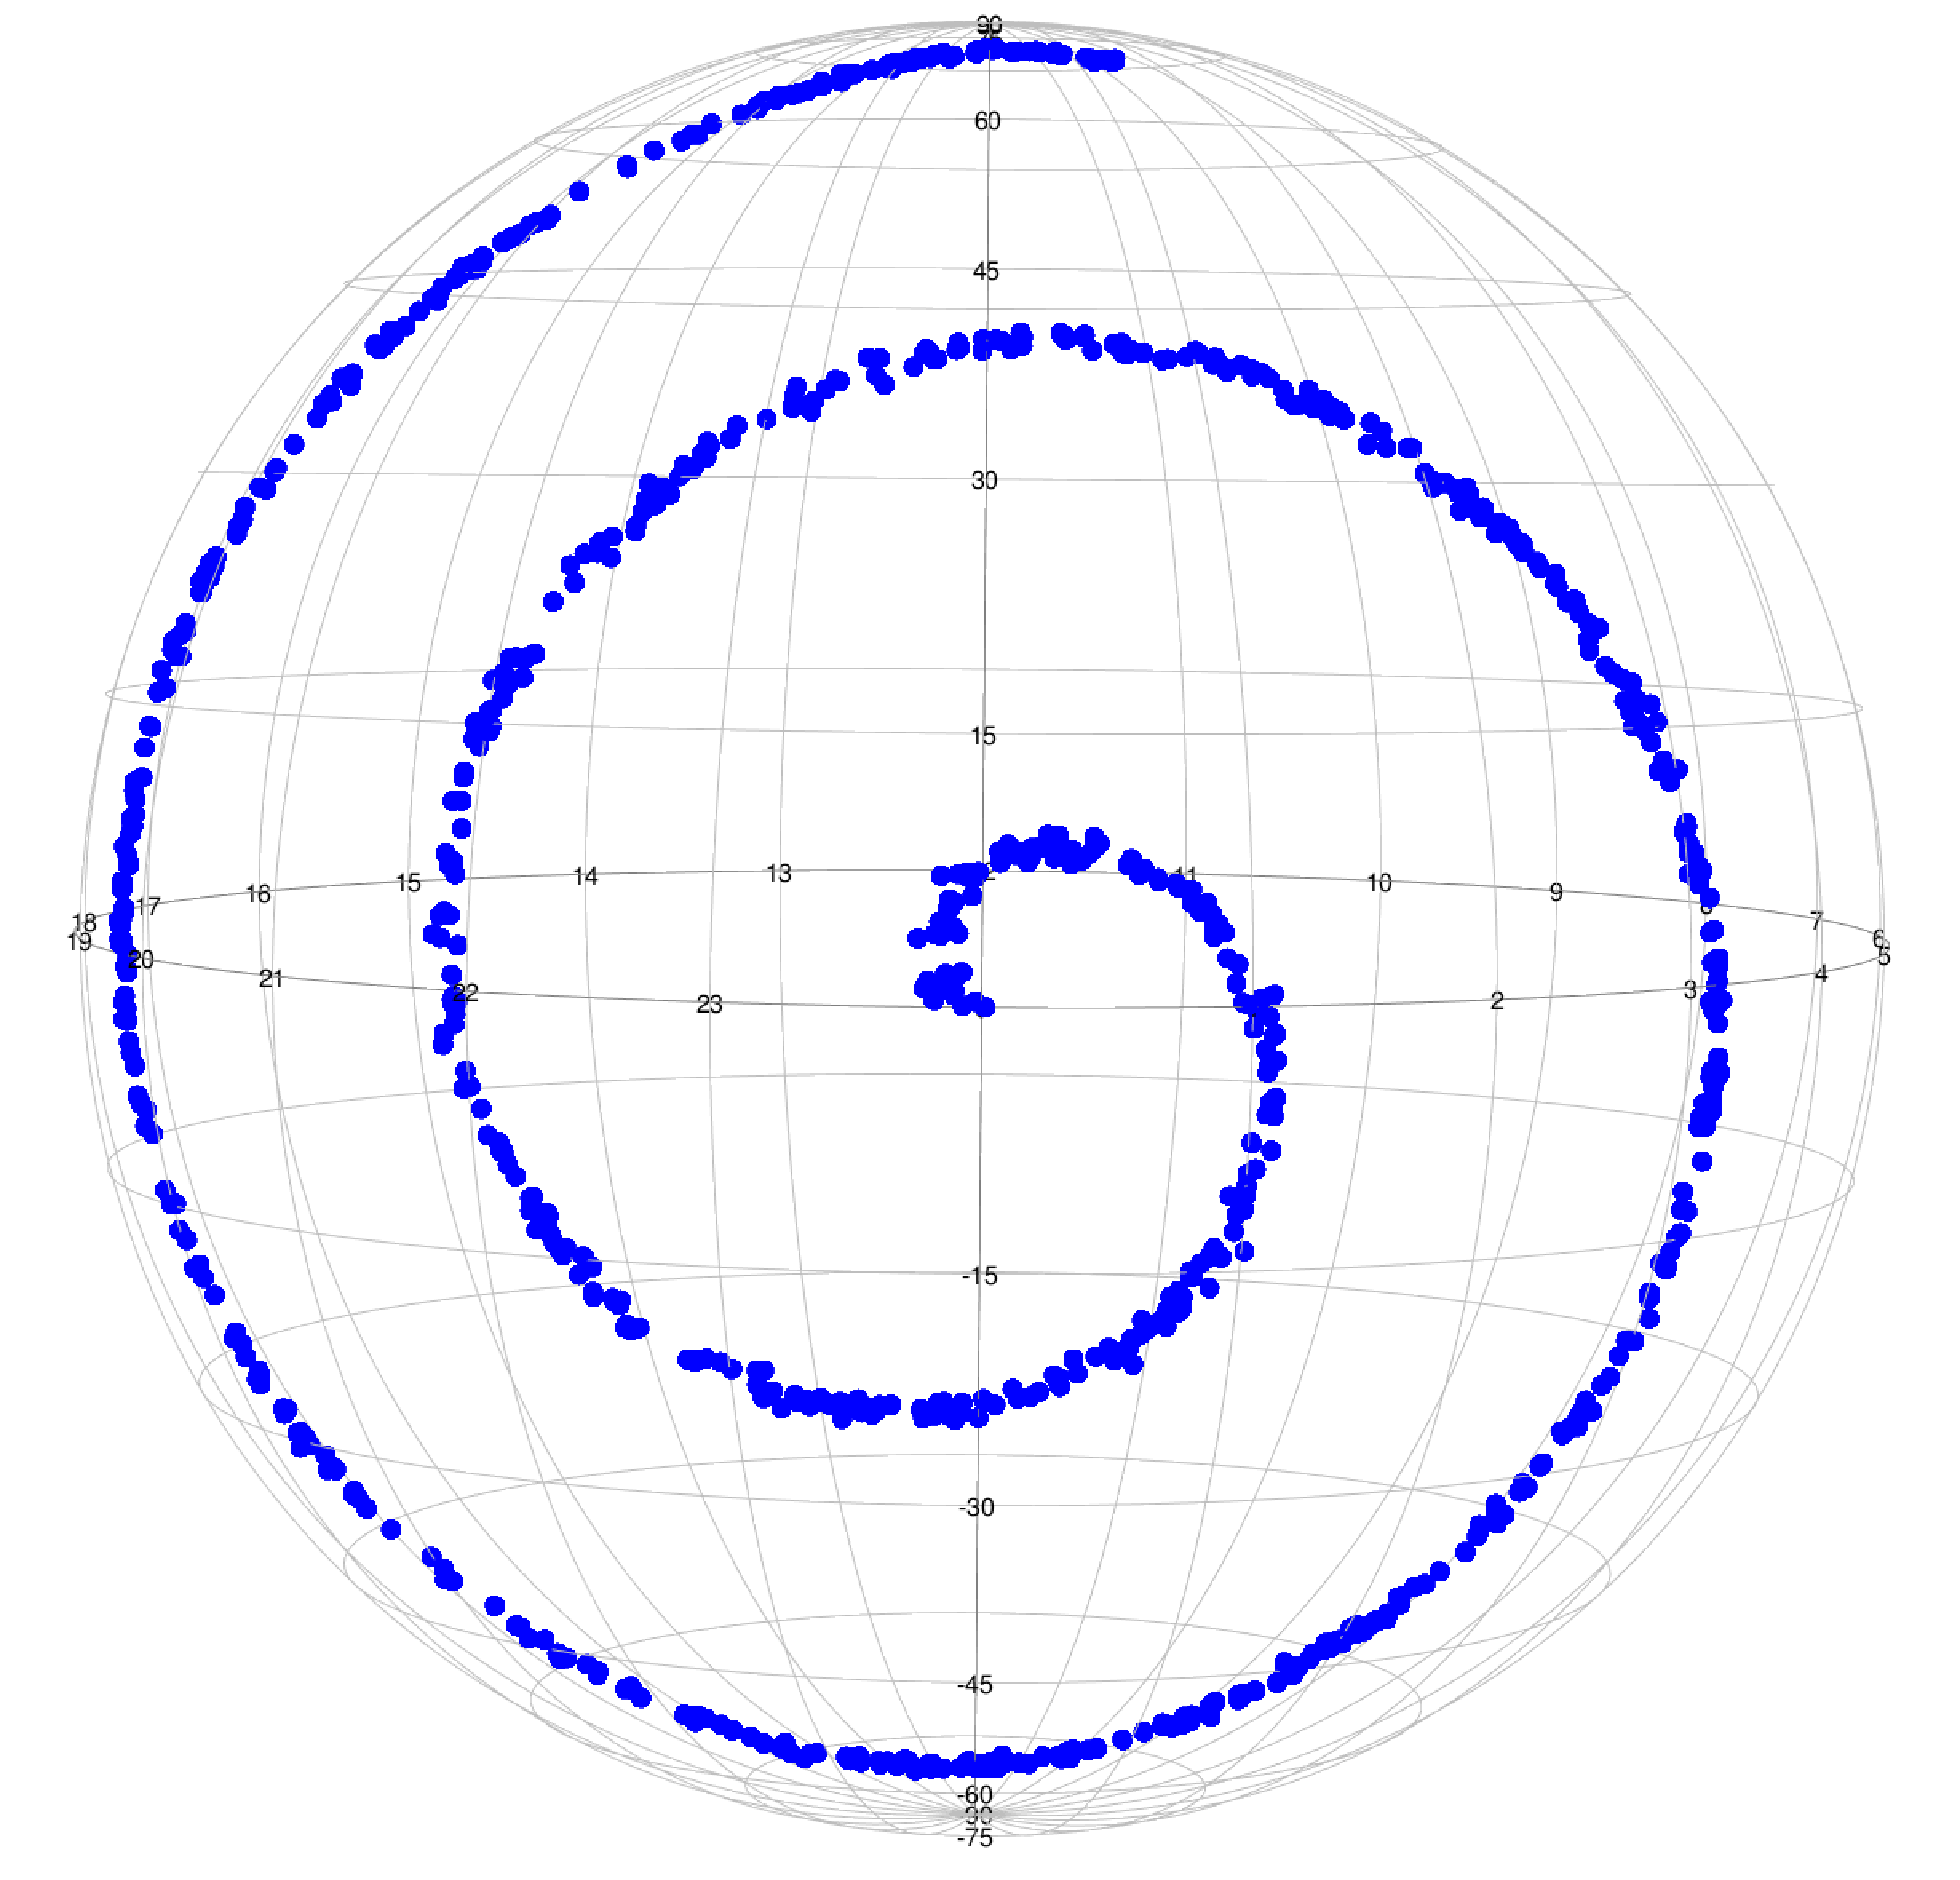
\includegraphics[scale=0.1]{figures/spiral.png}
    \hspace{0cm}
    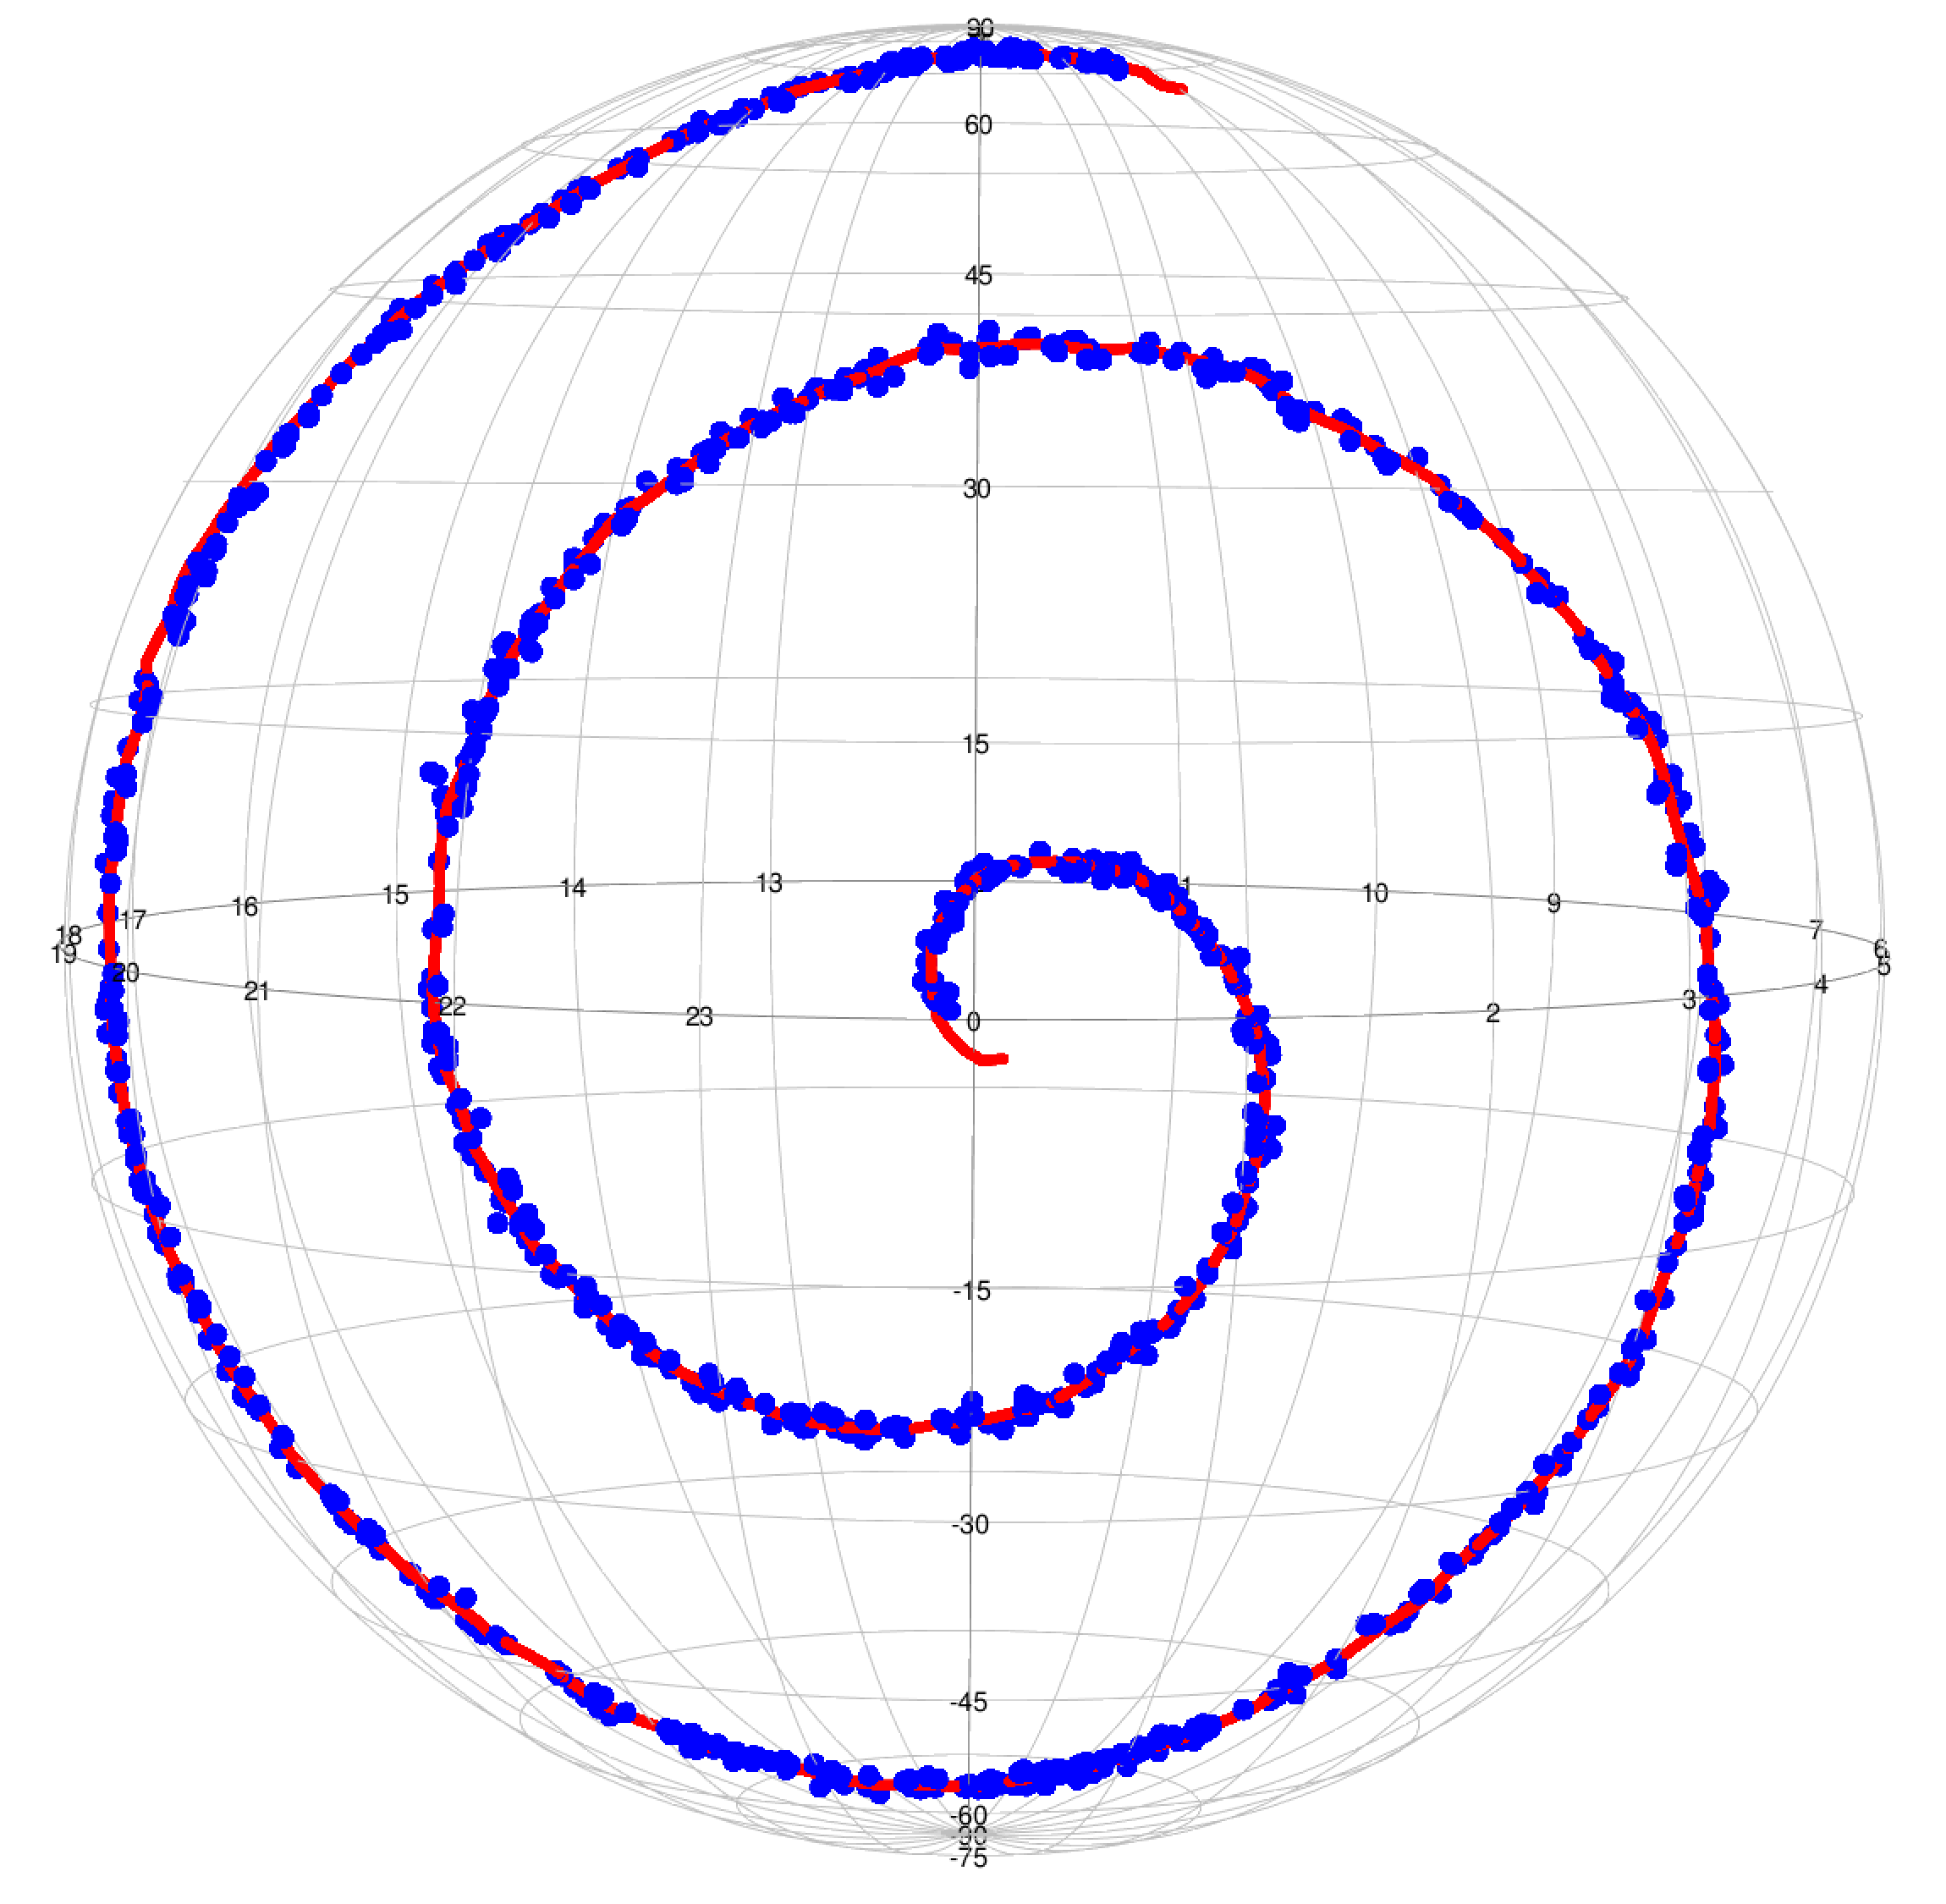
\includegraphics[scale=0.1]{figures/LPG(spiral).png}
    \hspace{0cm}
    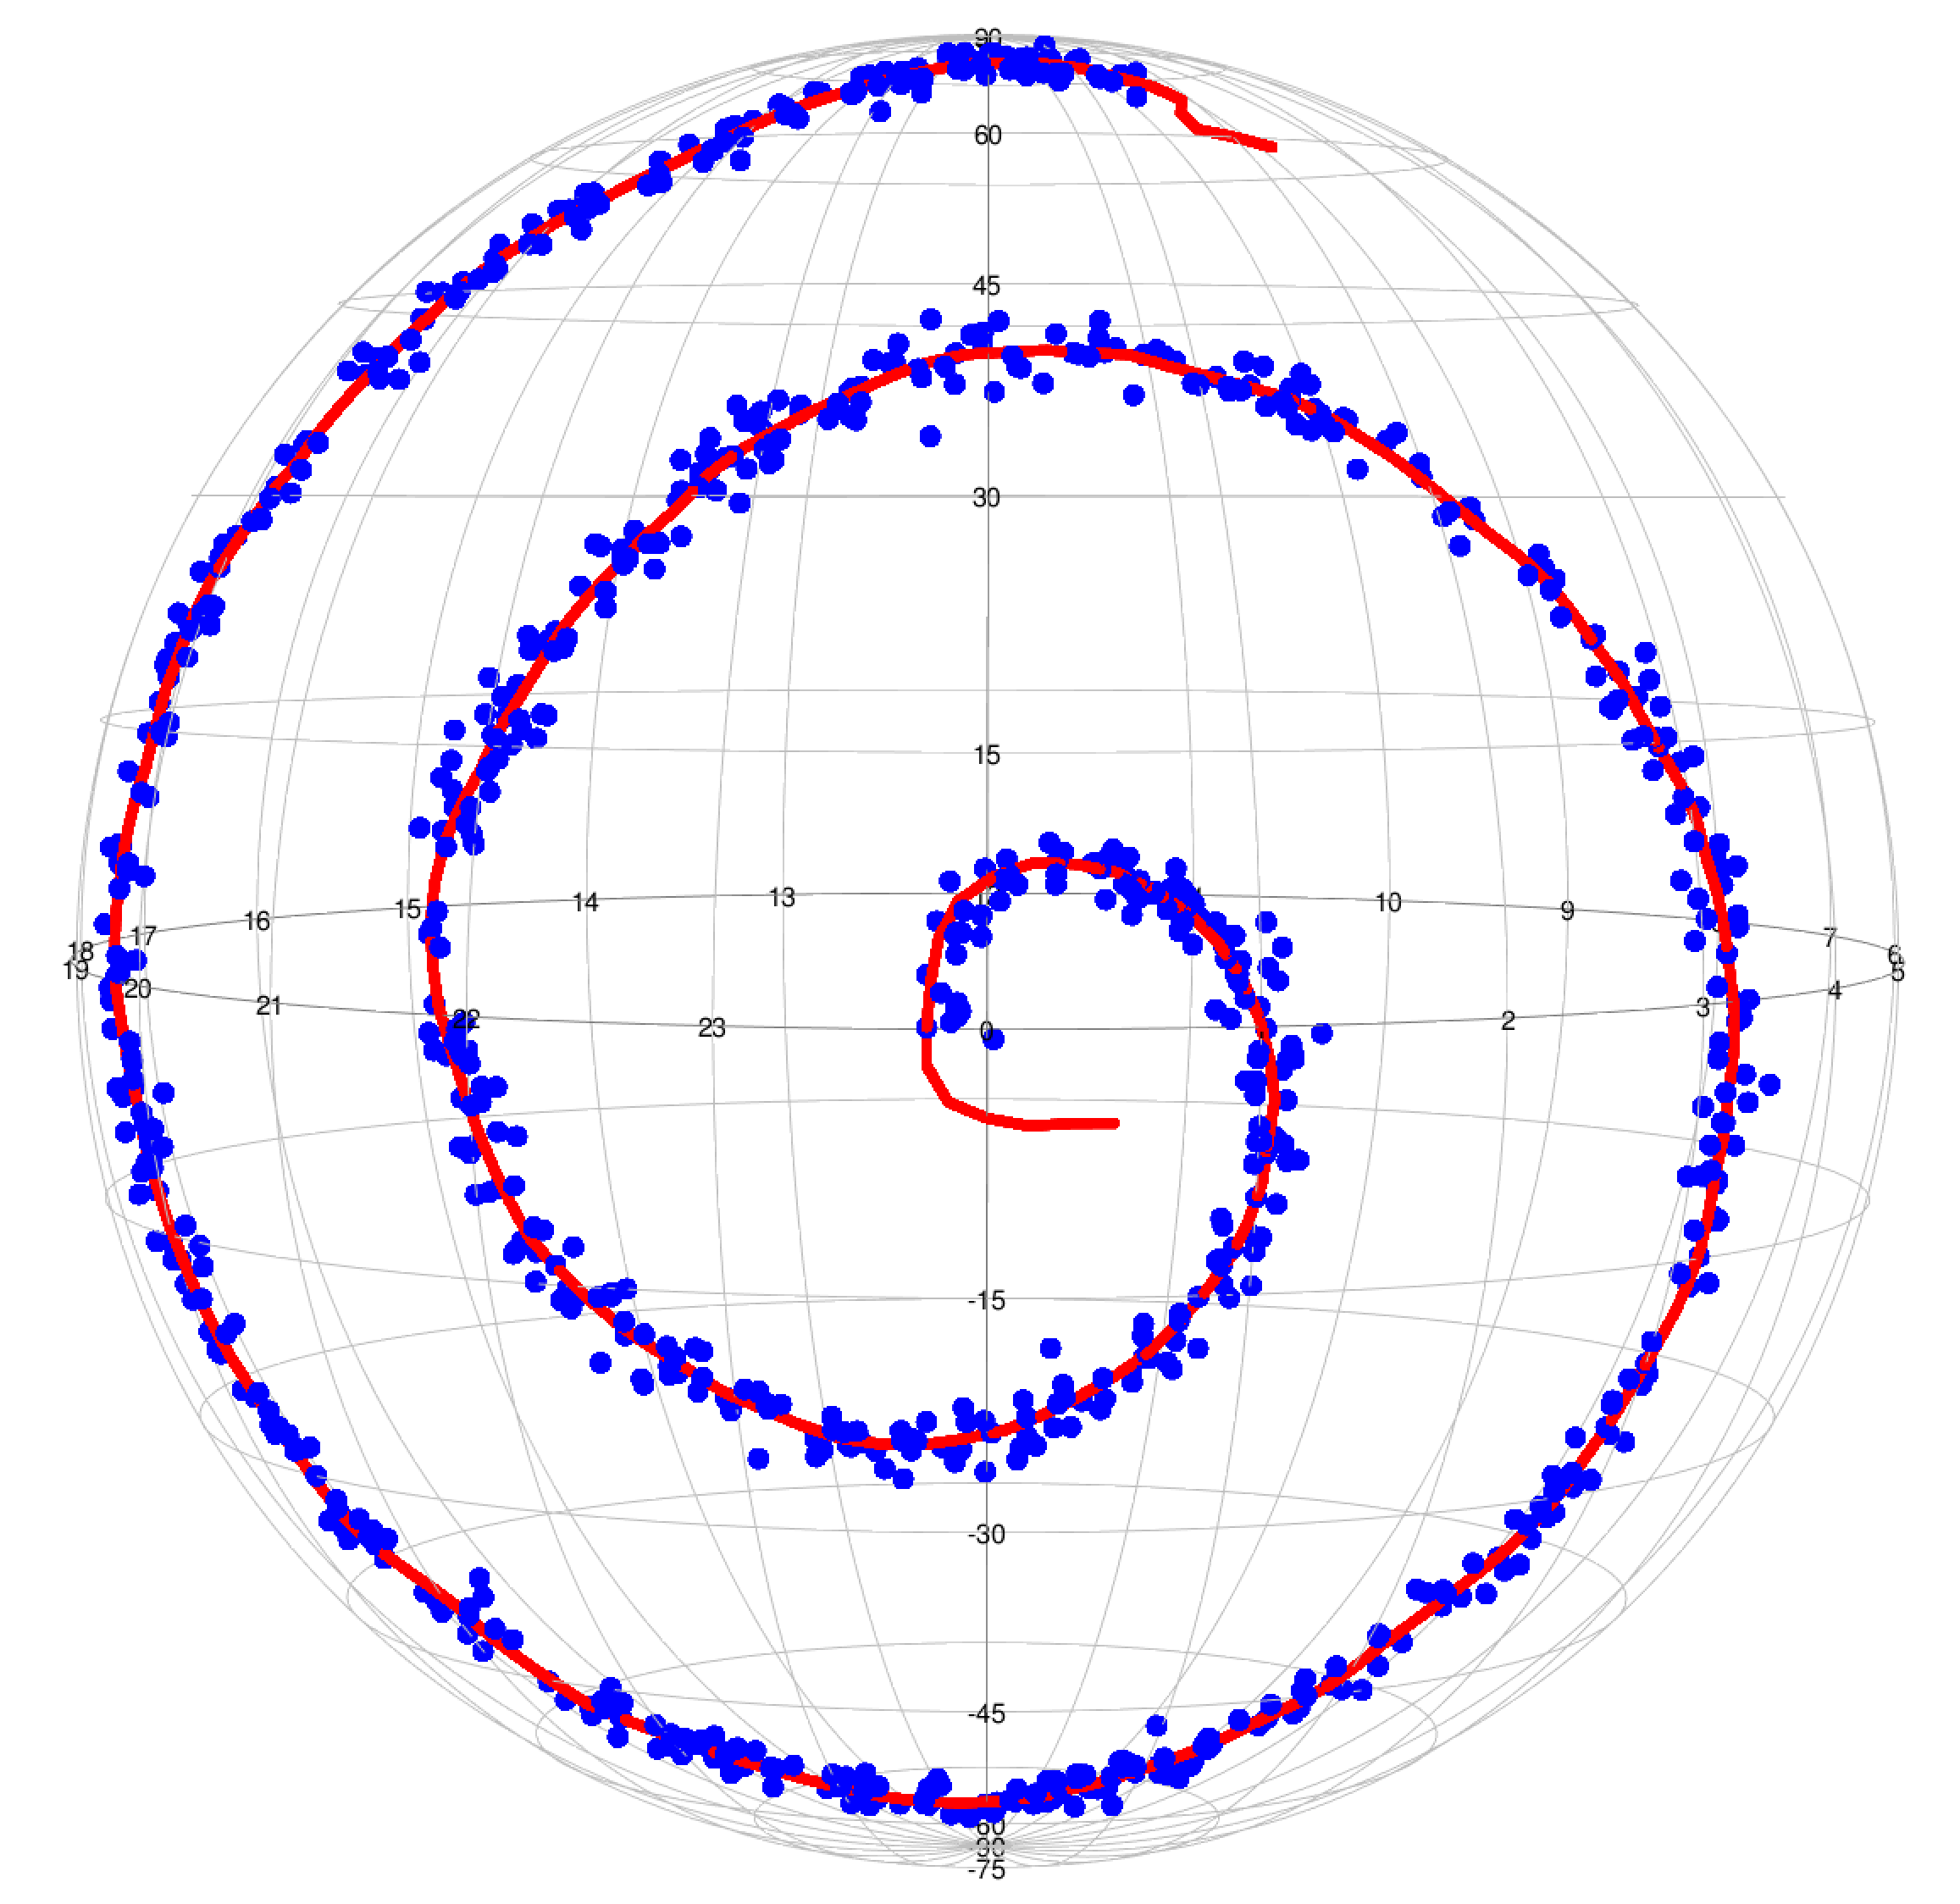
\includegraphics[scale=0.1]{figures/LPG(spiral_noisy).png}
    \caption{Left: Spiral data (blue) and the result (red) of LPG with $\mbox{scale}=0.06$ and $\mbox{nu}=0.1$. Right: Noisy spiral data (blue) and the result (red) of LPG with $\mbox{scale} = 0.12$ and $\mbox{nu} = 0.1$. Local principal geodesics represent the spiral patterns of the (noisy) spiral data. The larger the noise is, the larger scale is required.}
    \label{fig:spiral}
\end{figure}

\begin{example}
   #### example 2: zigzag data
   > set.seed(10)
   > n <- 50                                # the number of samples is 6 * n = 300
   > sigma1 <- 2; sigma2 <- 5               # noise levels                   
   > x1 <- x2 <- x3 <- x4 <- x5 <- x6 <- runif(n) * 20 - 20
   > y1 <- x1 + 20 + sigma1 * rnorm(n); y2 <- -x2 + 20 + sigma1 * rnorm(n)
   > y3 <- x3 + 60 + sigma1 * rnorm(n); y4 <- -x4 - 20 + sigma1 * rnorm(n)
   > y5 <- x5 - 20 + sigma1 * rnorm(n); y6 <- -x6 - 60 + sigma1 * rnorm(n)
   > x <- c(x1, x2, x3, x4, x5, x6); y <- c(y1, y2, y3, y4, y5, y6)
   > simul.zigzag1 <- cbind(x, y)
   ## plot the zigzag data
   > sphereplot::rgl.sphgrid(col.lat = 'black', col.long = 'black')
   > sphereplot::rgl.sphpoints(simul.zigzag1, radius = 1, col = 'blue', size = 12)
   ## implement the LPG to the zigzag data
   > LPG(simul.zigzag1, scale = 0.1, nu = 0.1, maxpt = 45, seed = 50)

   ## noisy zigzag data
   > set.seed(10)
   > z1 <- z2 <- z3 <- z4 <- z5 <- z6 <- runif(n) * 20 - 20
   > w1 <- z1 + 20 + sigma2 * rnorm(n); w2 <- -z2 + 20 + sigma2 * rnorm(n)
   > w3 <- z3 + 60 + sigma2 * rnorm(n); w4 <- -z4 - 20 + sigma2 * rnorm(n)
   > w5 <- z5 - 20 + sigma2 * rnorm(n); w6 <- -z6 - 60 + sigma2 * rnorm(n)
   > z <- c(z1, z2, z3, z4, z5, z6); w <- c(w1, w2, w3, w4, w5, w6)
   > simul.zigzag2 <- cbind(z, w)
   ## implement the LPG to the noisy zigzag data
   > LPG(simul.zigzag2, scale = 0.2, nu = 0.1, maxpt = 18, seed = 20)

\end{example}


\begin{figure}[h]
    \centering
    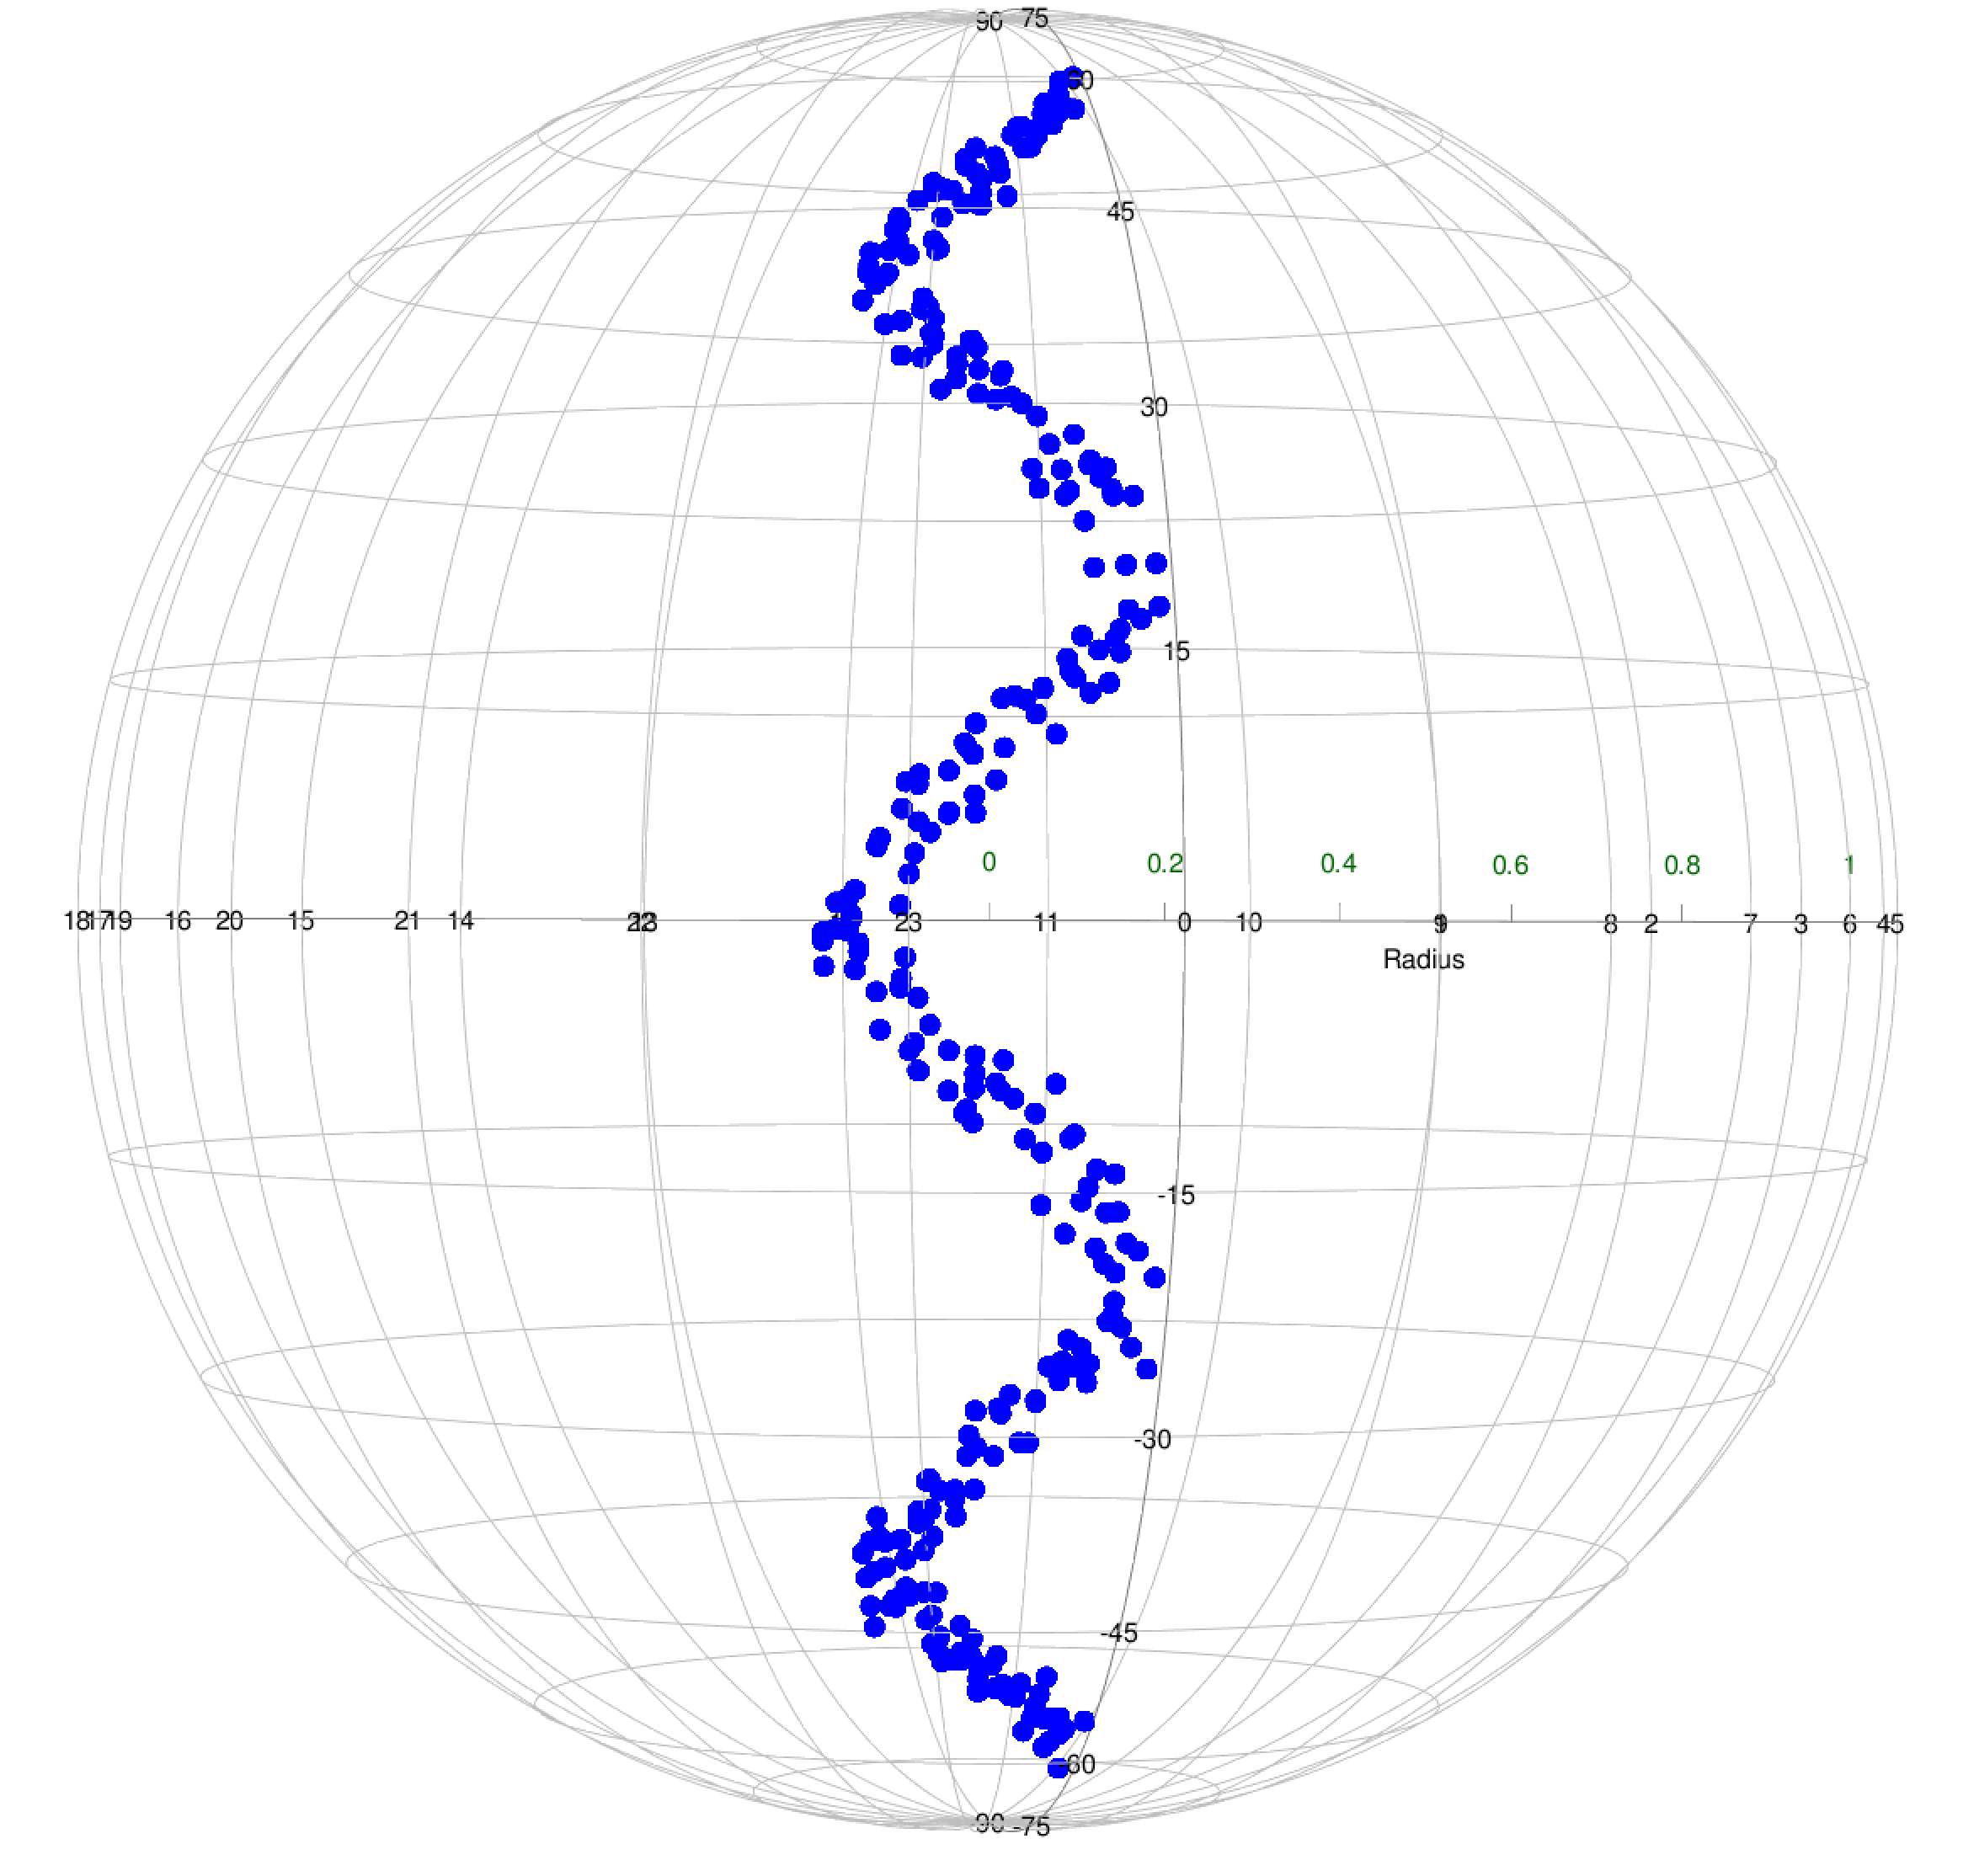
\includegraphics[scale=0.11]{figures/zigzag.png}
    \hspace{0cm}
    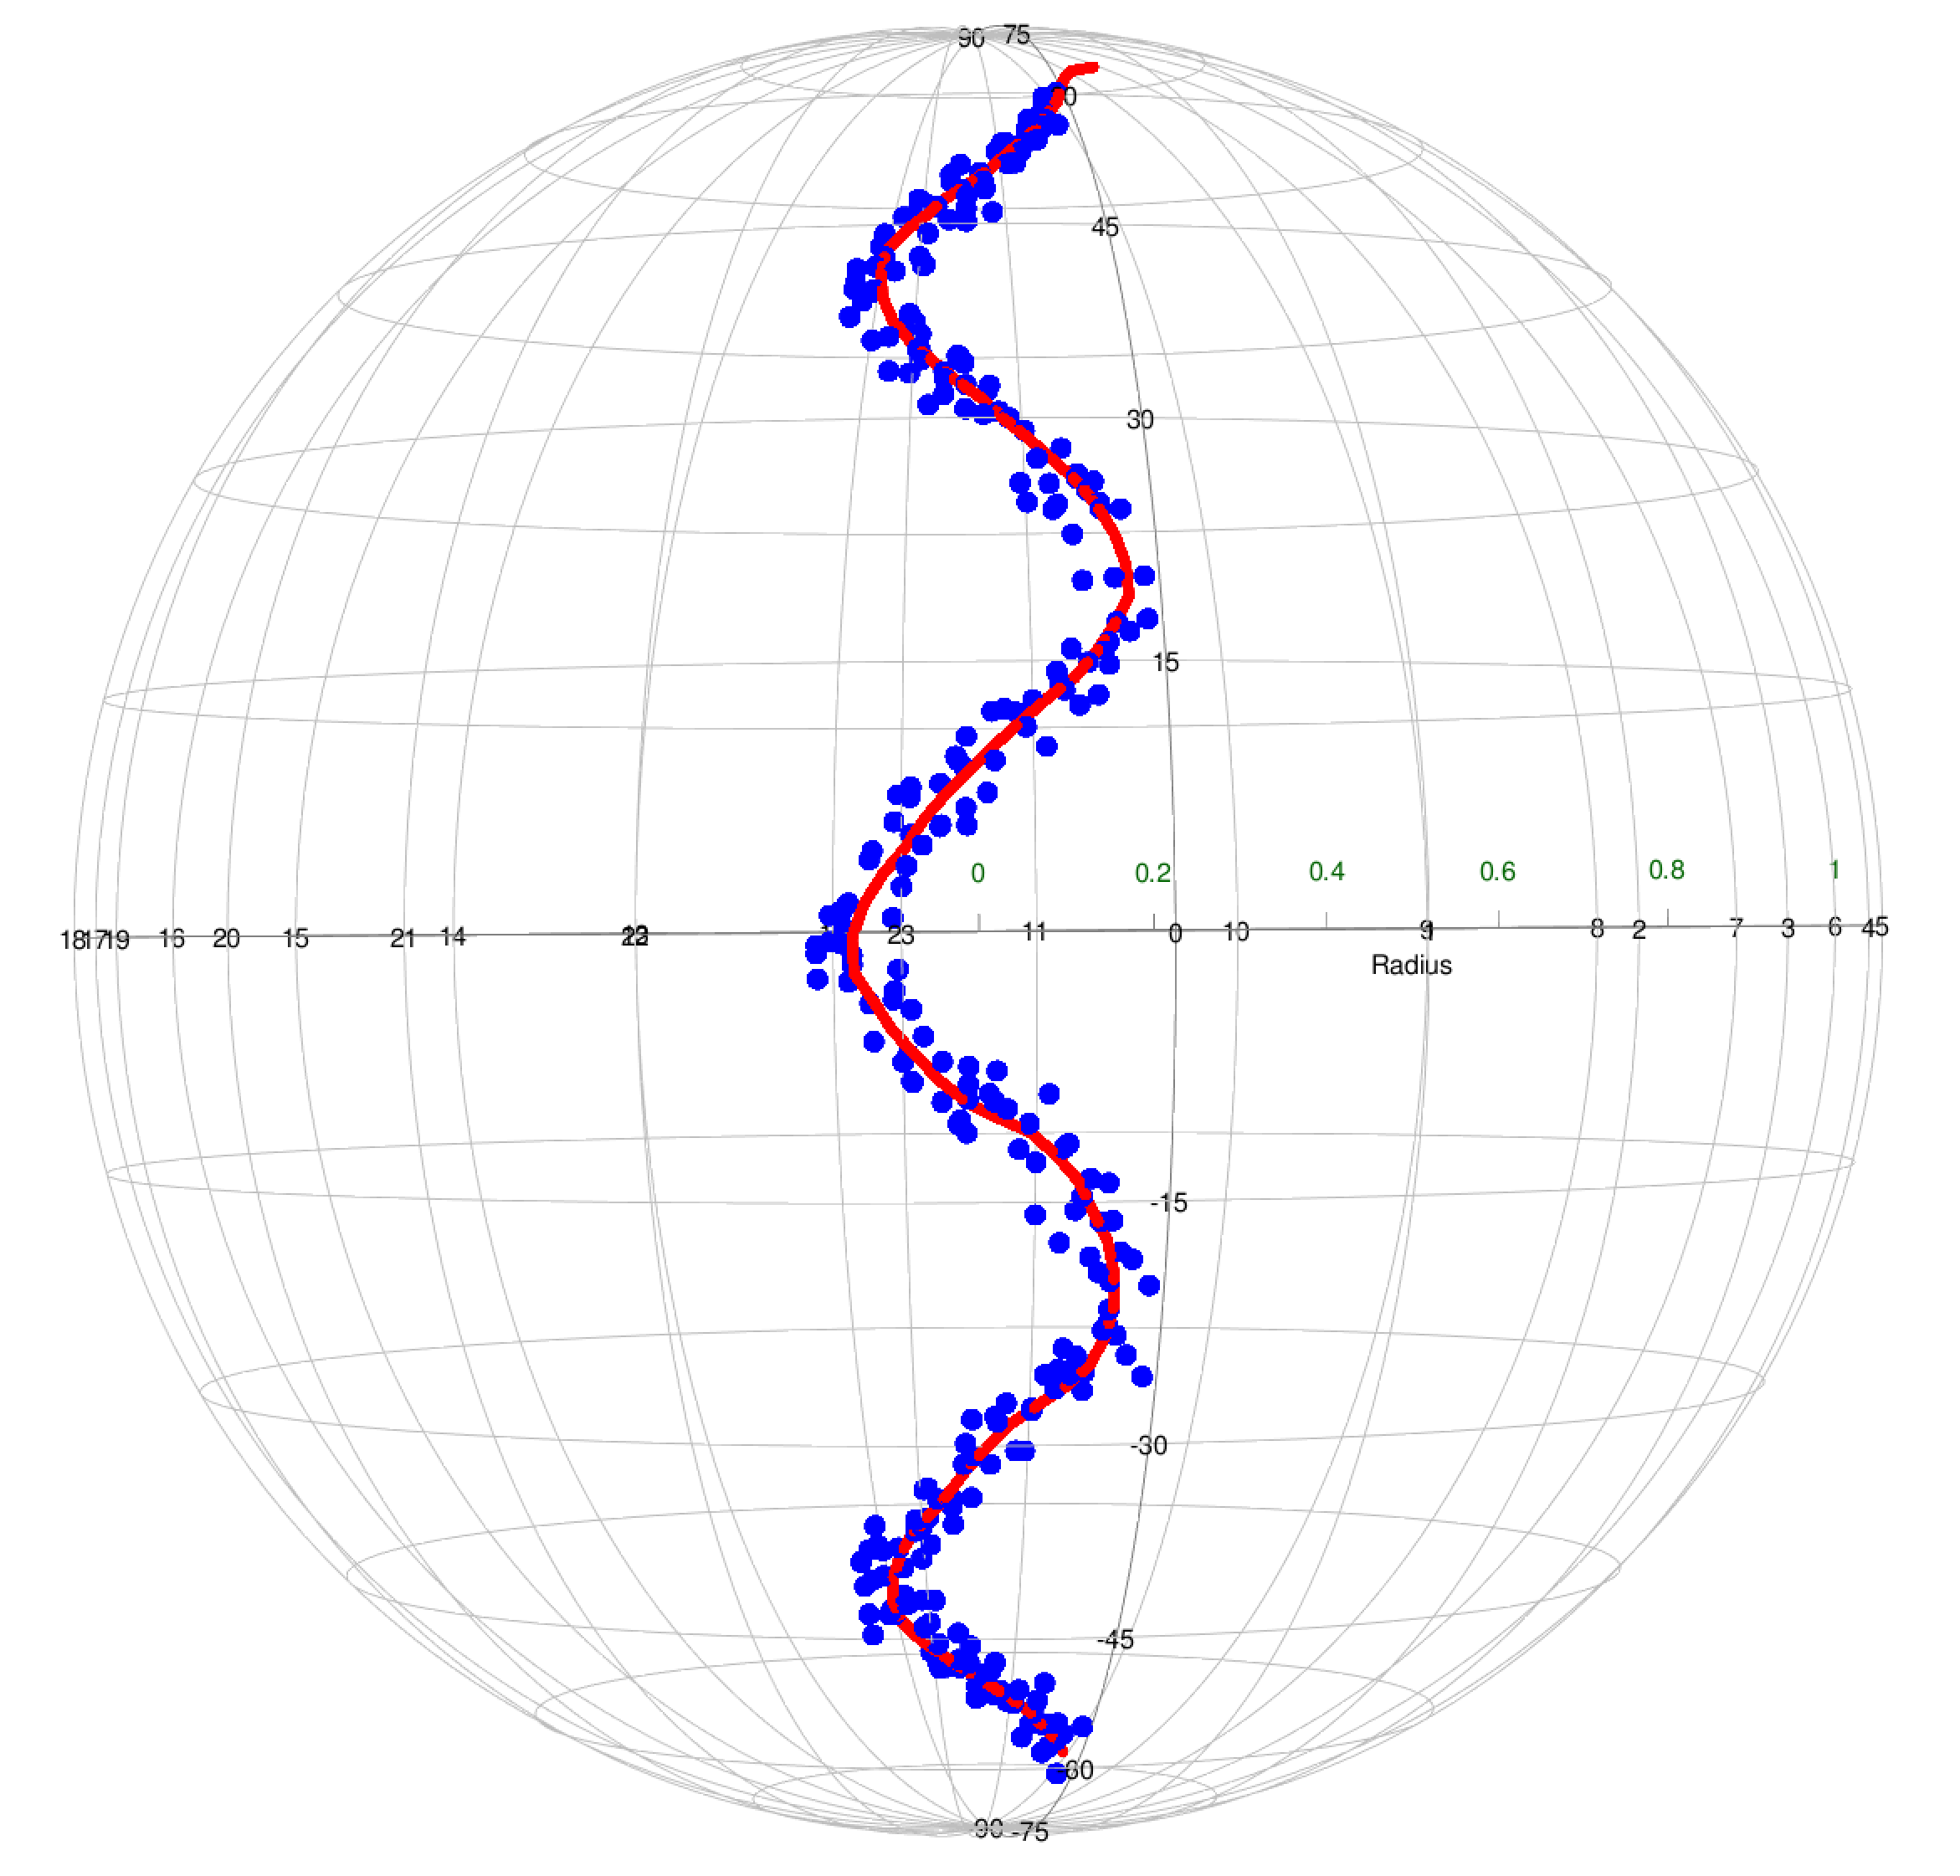
\includegraphics[scale=0.11]{figures/LPG(zigzag).png}
    \hspace{0cm}
    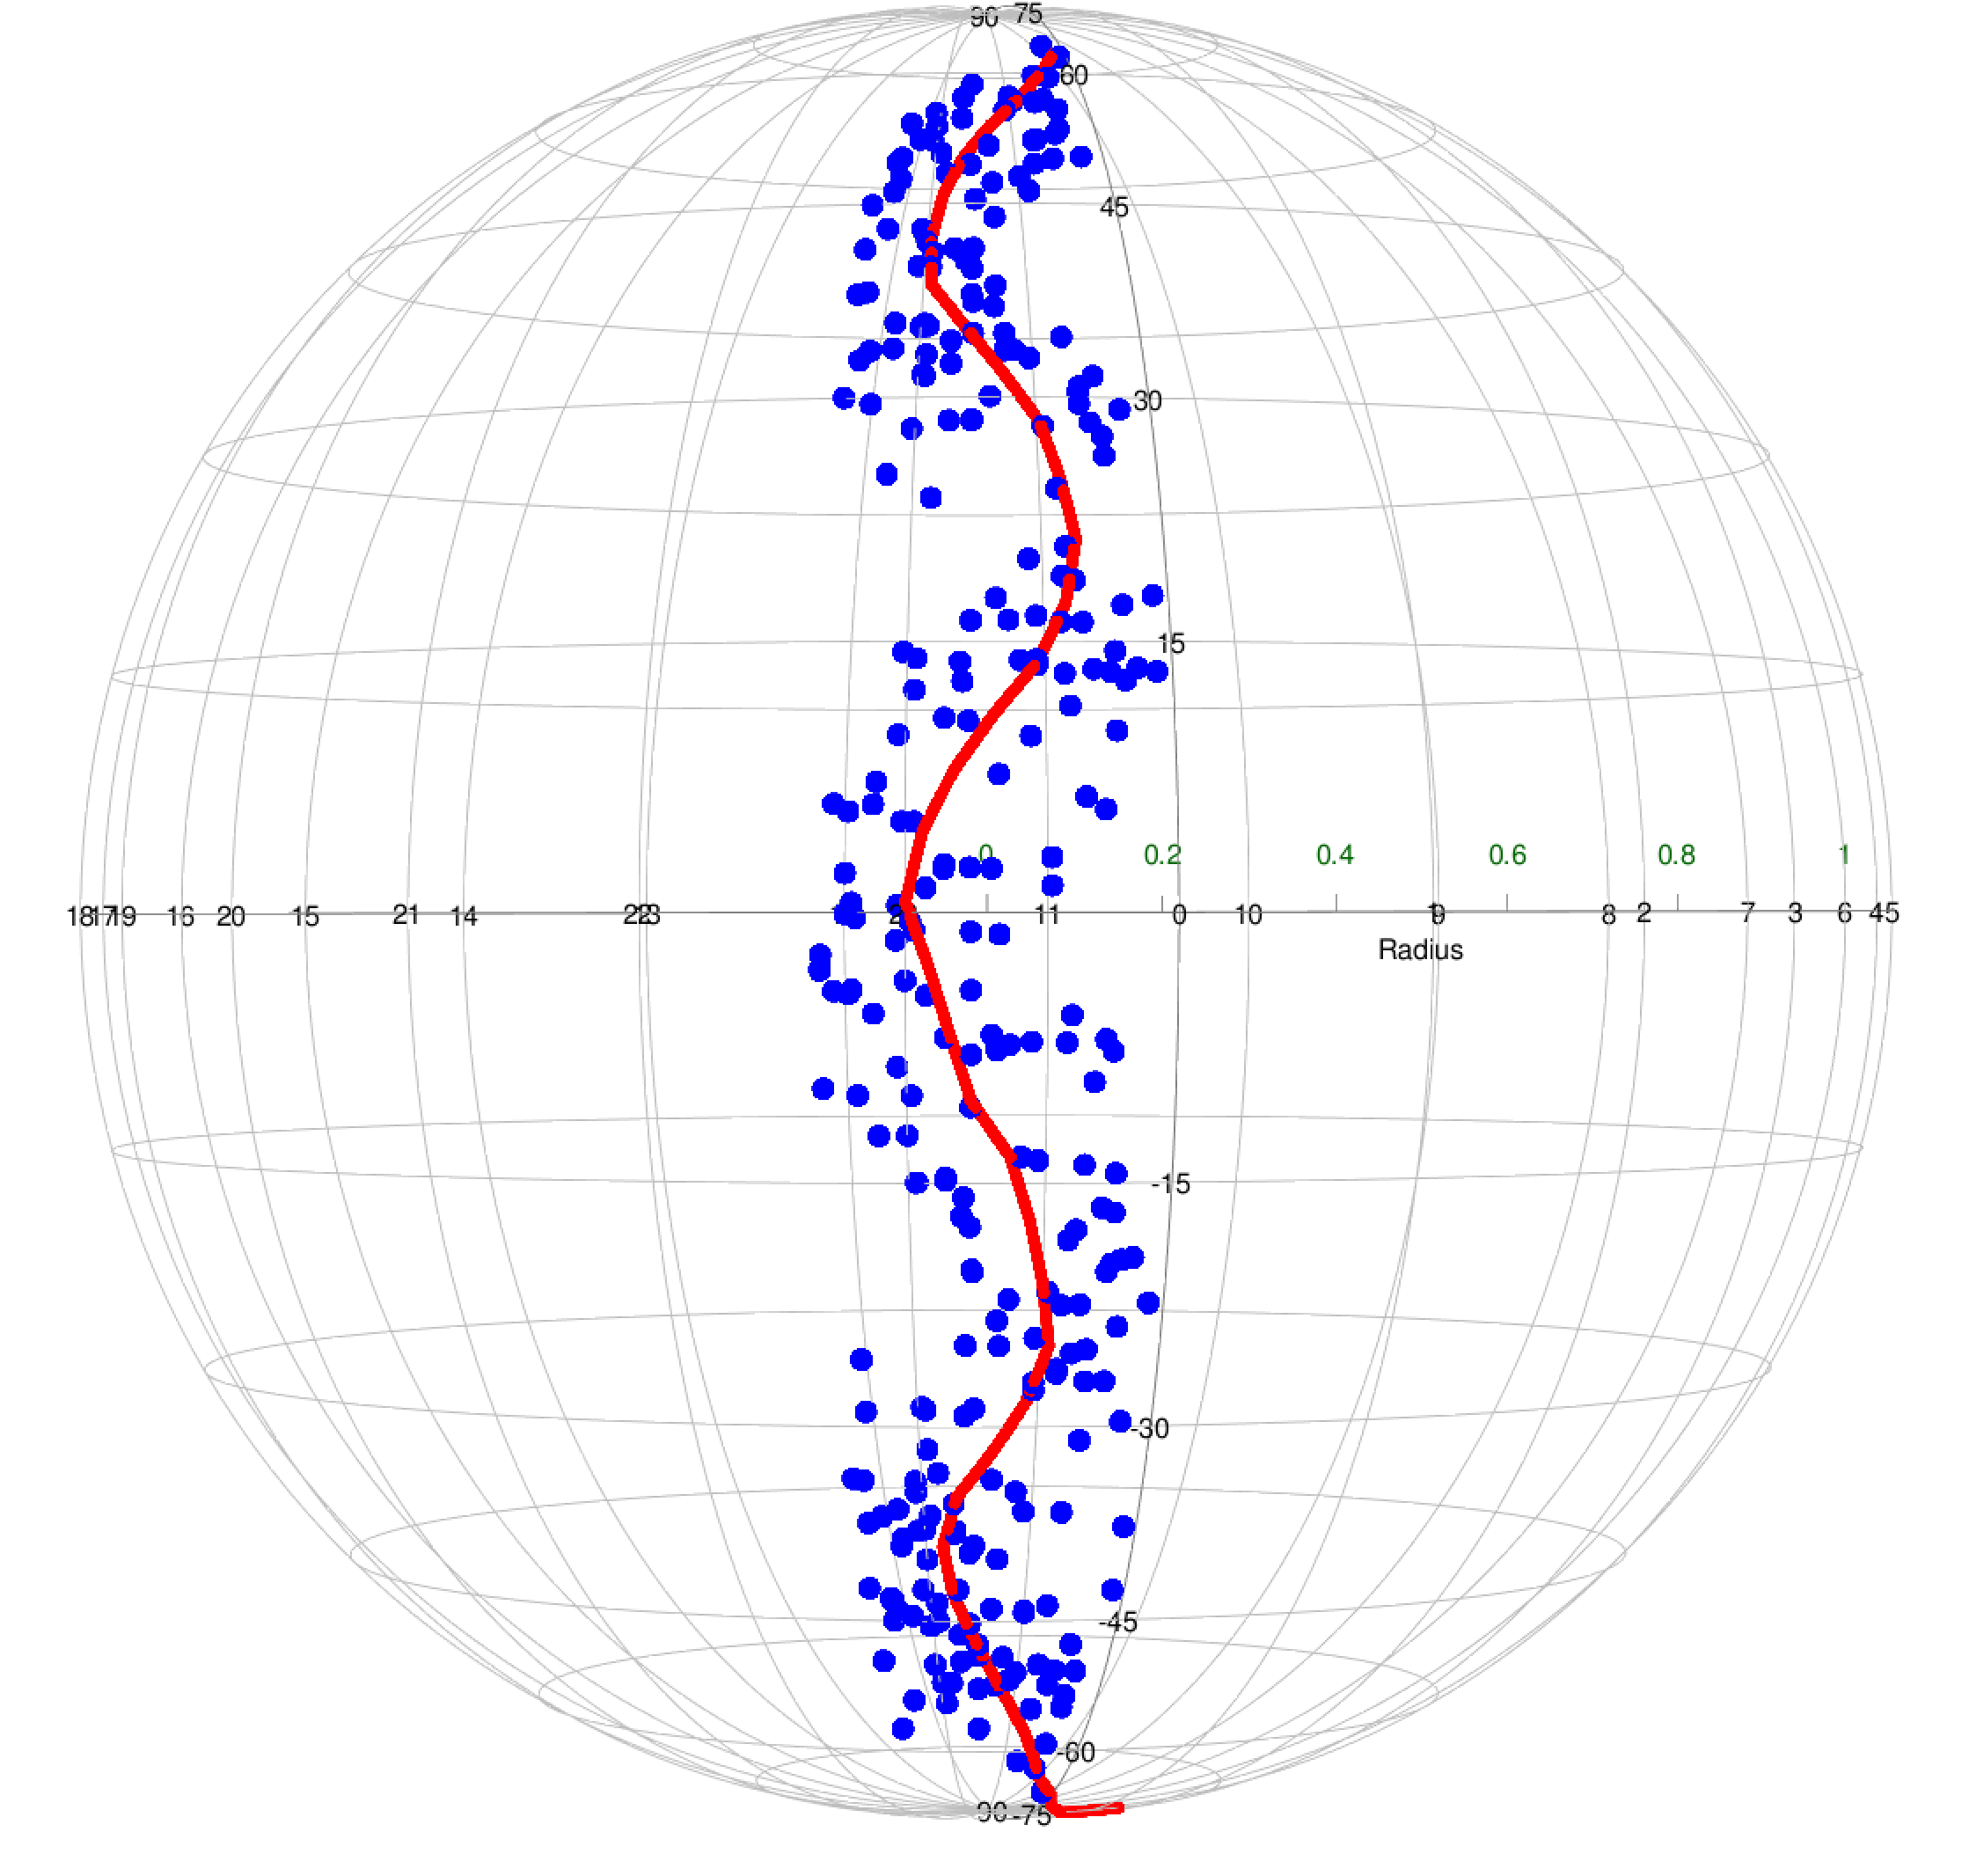
\includegraphics[scale=0.115]{figures/LPG(zigzag_noisy).png}
    \caption{Left: zigzag data (blue). Middle: zigzag data (blue) and the result (red) of with $\mbox{scale}=0.1$ and $\mbox{nu}=0.1$. Right: Noisy zigzag data (blue) and the result (red) of LPG with $\mbox{scale}=0.2, ~ \mbox{and} ~ \mbox{nu}=0.1$. Local principal geodesics extract the zigzag structures of the (noisy) zigzag data properly. The larger the noise is, the larger scale is needed.}
    \label{fig:zigzag}
\end{figure}

Note that the \code{LPG()} function may return several curves. We now implement the function in a complex simulation dataset composed of several curves. As shown in the left panel of Figure~\ref{fig:tree}, the tree object has twenty-six geodesic (linear) structures consisting of one stem, five branches, and twenty subbranches. It is not informative to show the generating formula for the tree dataset. Instead, we provide its generating code with explanatory notes as follows.

\begin{example}
  #### example 3: tree dataset
  ## the tree dataset consists of stem, branches and subbranches
  ## generate stem
  > set.seed(10)
  > n1 <- 200; n2 <- 100; n3 <- 15     # the number of samples in
                                       # a stem, a branch, and a subbrach
  > sigma1 <- 0.1; sigma2 <- 0.05; sigma3 <- 0.01          # noise levels
  > noise1 <- sigma1 * rnorm(n1); noise2 <- sigma2 * rnorm(n2)
  > noise3 <- sigma3 * rnorm(n3)
  > l1 <- 70; l2 <- 20; l3 <- 1        # length of stem, branches, and subbranches
  > rep1 <- l1 * runif(n1)             # repeated part of stem
  > stem <- cbind(0 + noise1, rep1 - 10)
  ## generate branch
  > rep2 <- l2 * runif(n2)             # repeated part of branch
  > branch1 <- cbind(-rep2, rep2 + 10 + noise2); branch2 <- cbind(rep2, rep2 + noise2)
  > branch3 <- cbind(rep2, rep2 + 20 + noise2)
  > branch4 <- cbind(rep2, rep2 + 40 + noise2)
  > branch5 <- cbind(-rep2, rep2 + 30 + noise2)
  > branch <- rbind(branch1, branch2, branch3, branch4, branch5)
  ## generate subbranches
  > rep3 <- l3 * runif(n3)             # repeated part in subbranches
  > branches1 <- cbind(rep3 - 10, rep3 + 20 + noise3)
  > branches2 <- cbind(-rep3 + 10, rep3 + 10 + noise3)
  > branches3 <- cbind(rep3 - 14, rep3 + 24 + noise3)
  > branches4 <- cbind(-rep3 + 14, rep3 + 14 + noise3)
  > branches5 <- cbind(-rep3 - 12, -rep3 + 22 + noise3)
  > branches6 <- cbind(rep3 + 12, -rep3 + 12 + noise3)
  > branches7 <- cbind(-rep3 - 16, -rep3 + 26 + noise3)
  > branches8 <- cbind(rep3 + 16, -rep3 + 16 + noise3)
  > branches9 <- cbind(rep3 + 10, -rep3 + 50 + noise3)
  > branches10 <- cbind(-rep3 - 10, -rep3 + 40 + noise3)
  > branches11 <- cbind(-rep3 + 12, rep3 + 52 + noise3)
  > branches12 <- cbind(rep3 - 12, rep3 + 42 + noise3)
  > branches13 <- cbind(rep3 + 14, -rep3 + 54 + noise3)
  > branches14 <- cbind(-rep3 - 14, -rep3 + 44 + noise3)
  > branches15 <- cbind(-rep3 + 16, rep3 + 56 + noise3)
  > branches16 <- cbind(rep3 - 16, rep3 + 46 + noise3)
  > branches17 <- cbind(-rep3 + 10, rep3 + 30 + noise3)
  > branches18 <- cbind(-rep3 + 14, rep3 + 34 + noise3)
  > branches19 <- cbind(rep3 + 16, -rep3 + 36 + noise3)
  > branches20 <- cbind(rep3 + 12, -rep3 + 32 + noise3)
  > sub.branches <- rbind(branches1, branches2, branches3, branches4, branches5,
  + branches6, branches7, branches8, branches9, branches10, branches11, branches12,
  + branches13, branches14, branches15, branches16, branches17, branches18,
  + branches19, branches20)
  ## tree dataset consists of stem, branch, and subbranches
  > tree <- rbind(stem, branch, sub.branches)
  ## plot the tree dataset
  > sphereplot::rgl.sphgrid(col.lat = 'black', col.long = 'black')
  > sphereplot::rgl.sphpoints(tree, radius = 1, col = 'blue', size = 12)
  ## implement the LPG function to the tree dataset
  > LPG(tree, scale = 0.03, nu = 0.2, seed = 10)
\end{example}


\begin{figure}[h]
    \centering
    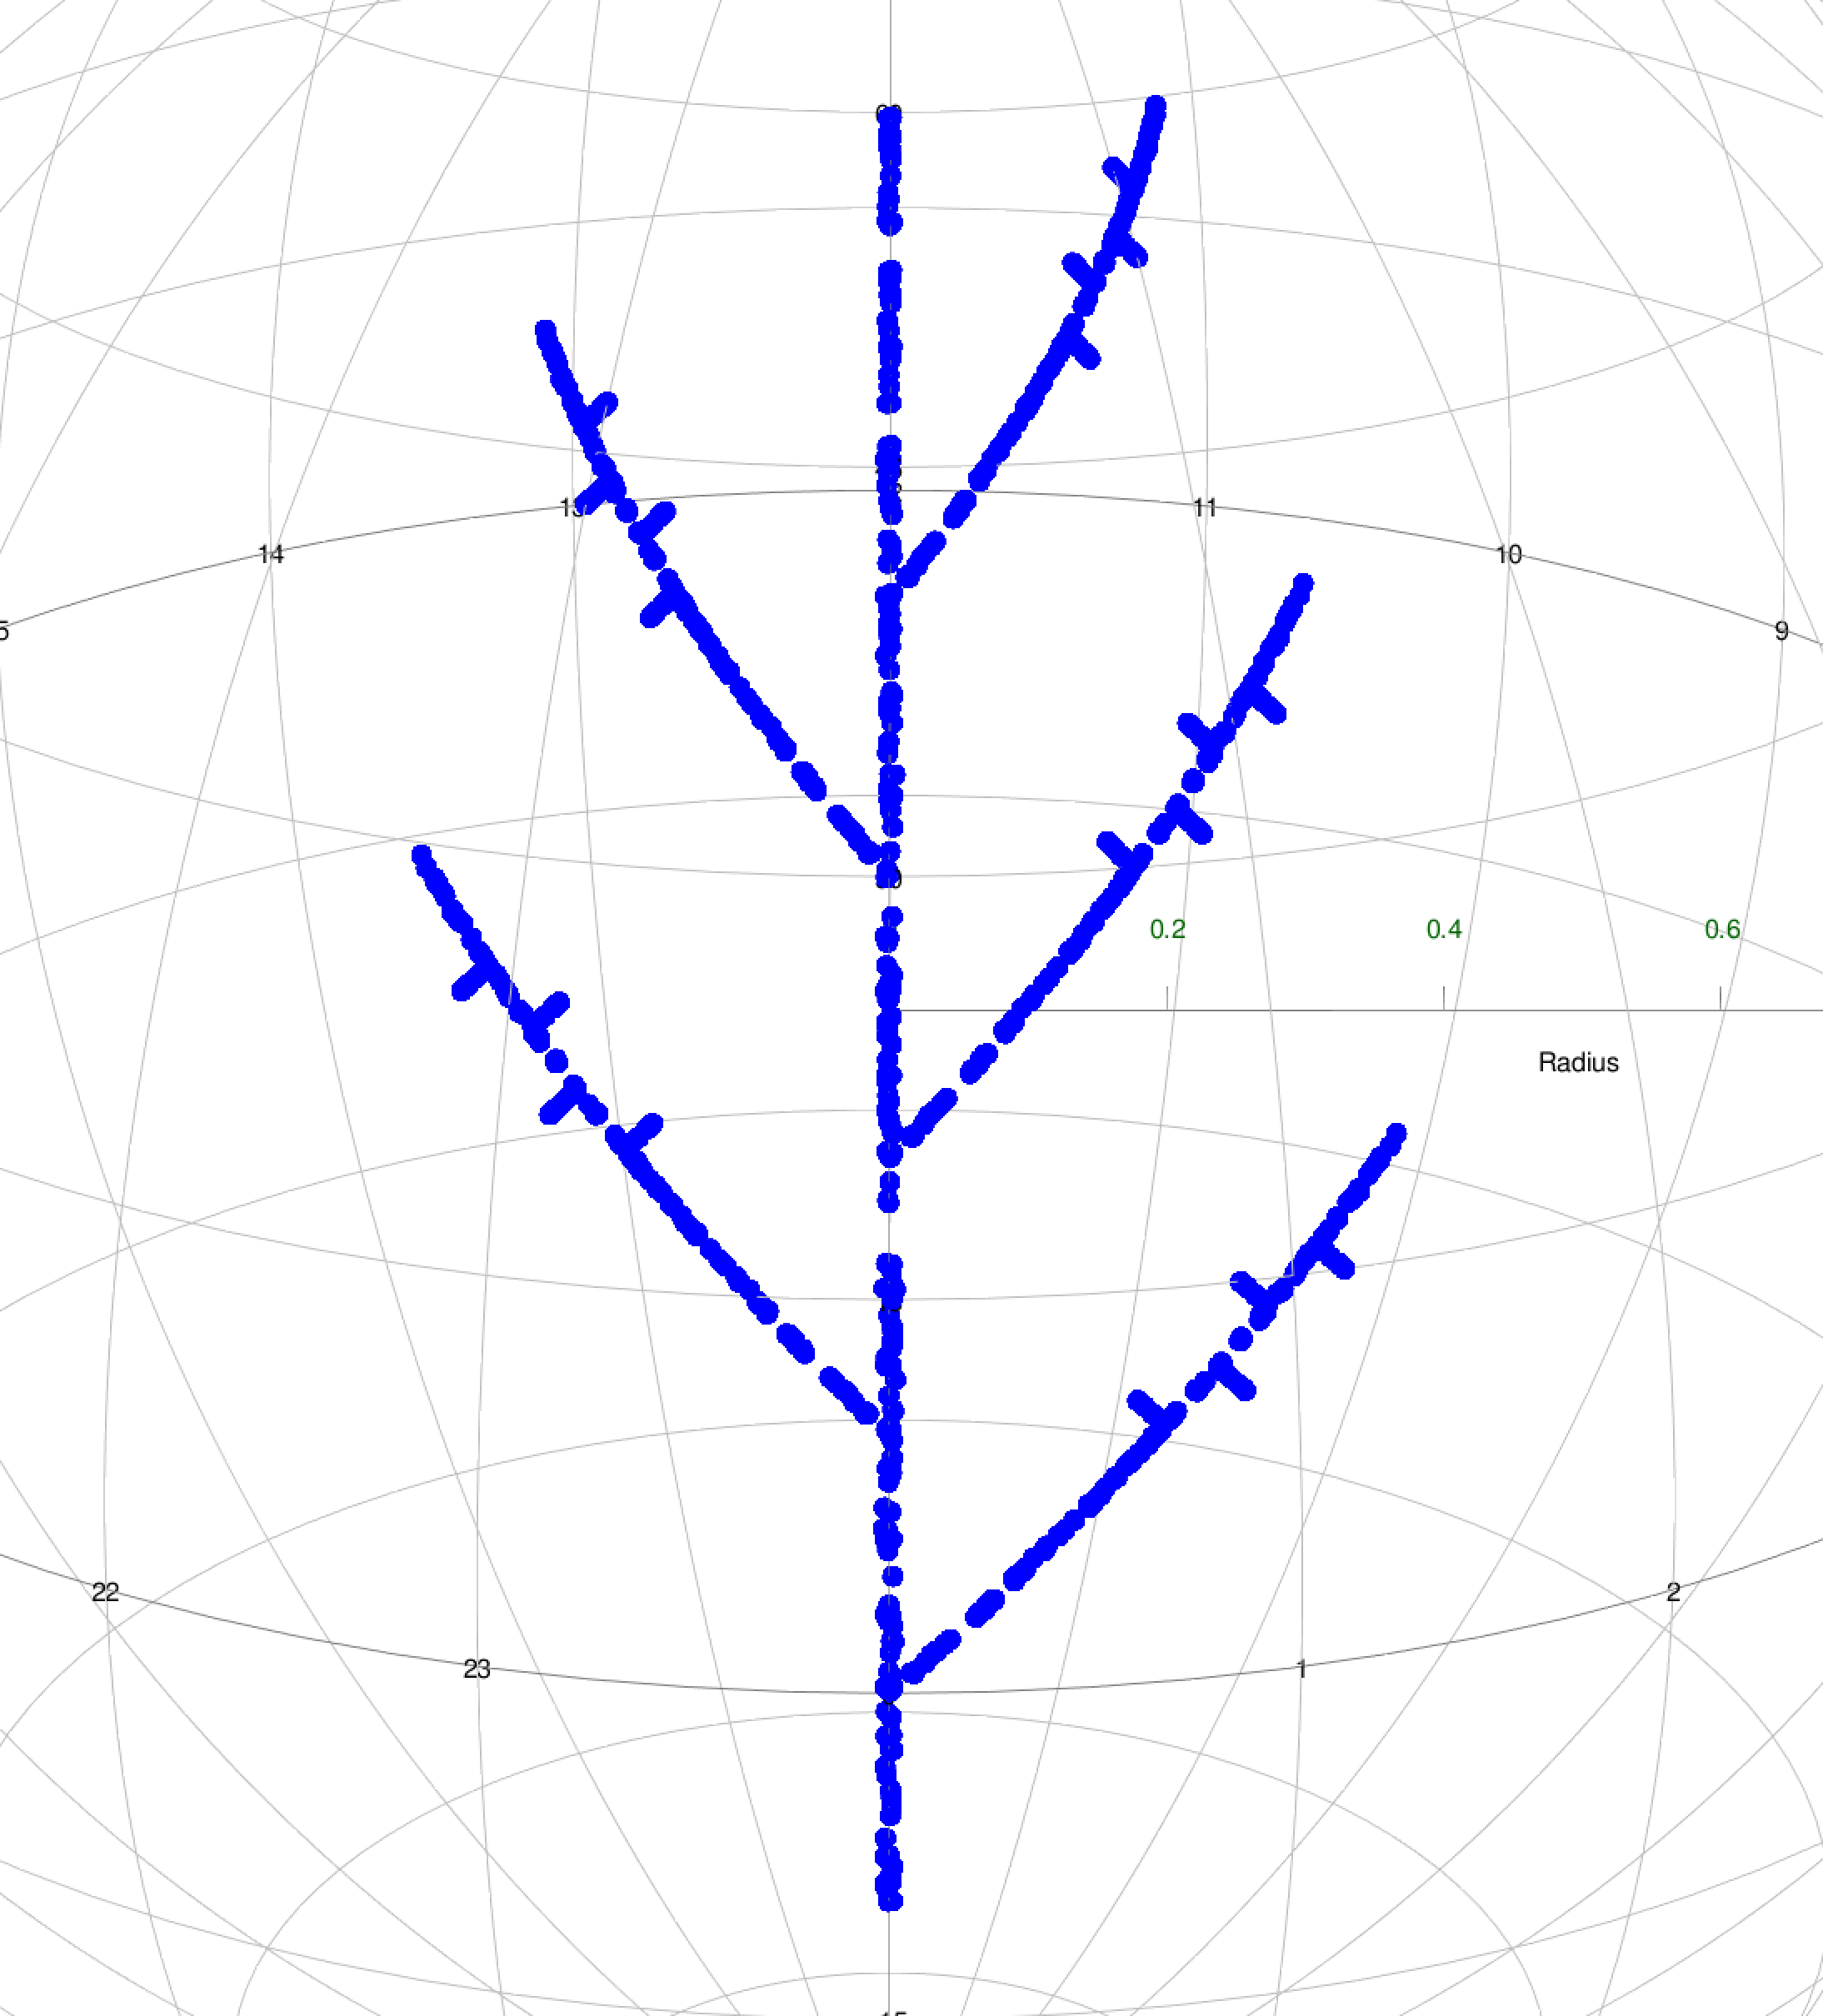
\includegraphics[scale=0.125]{figures/tree.png}
    \hspace{1.5cm}
    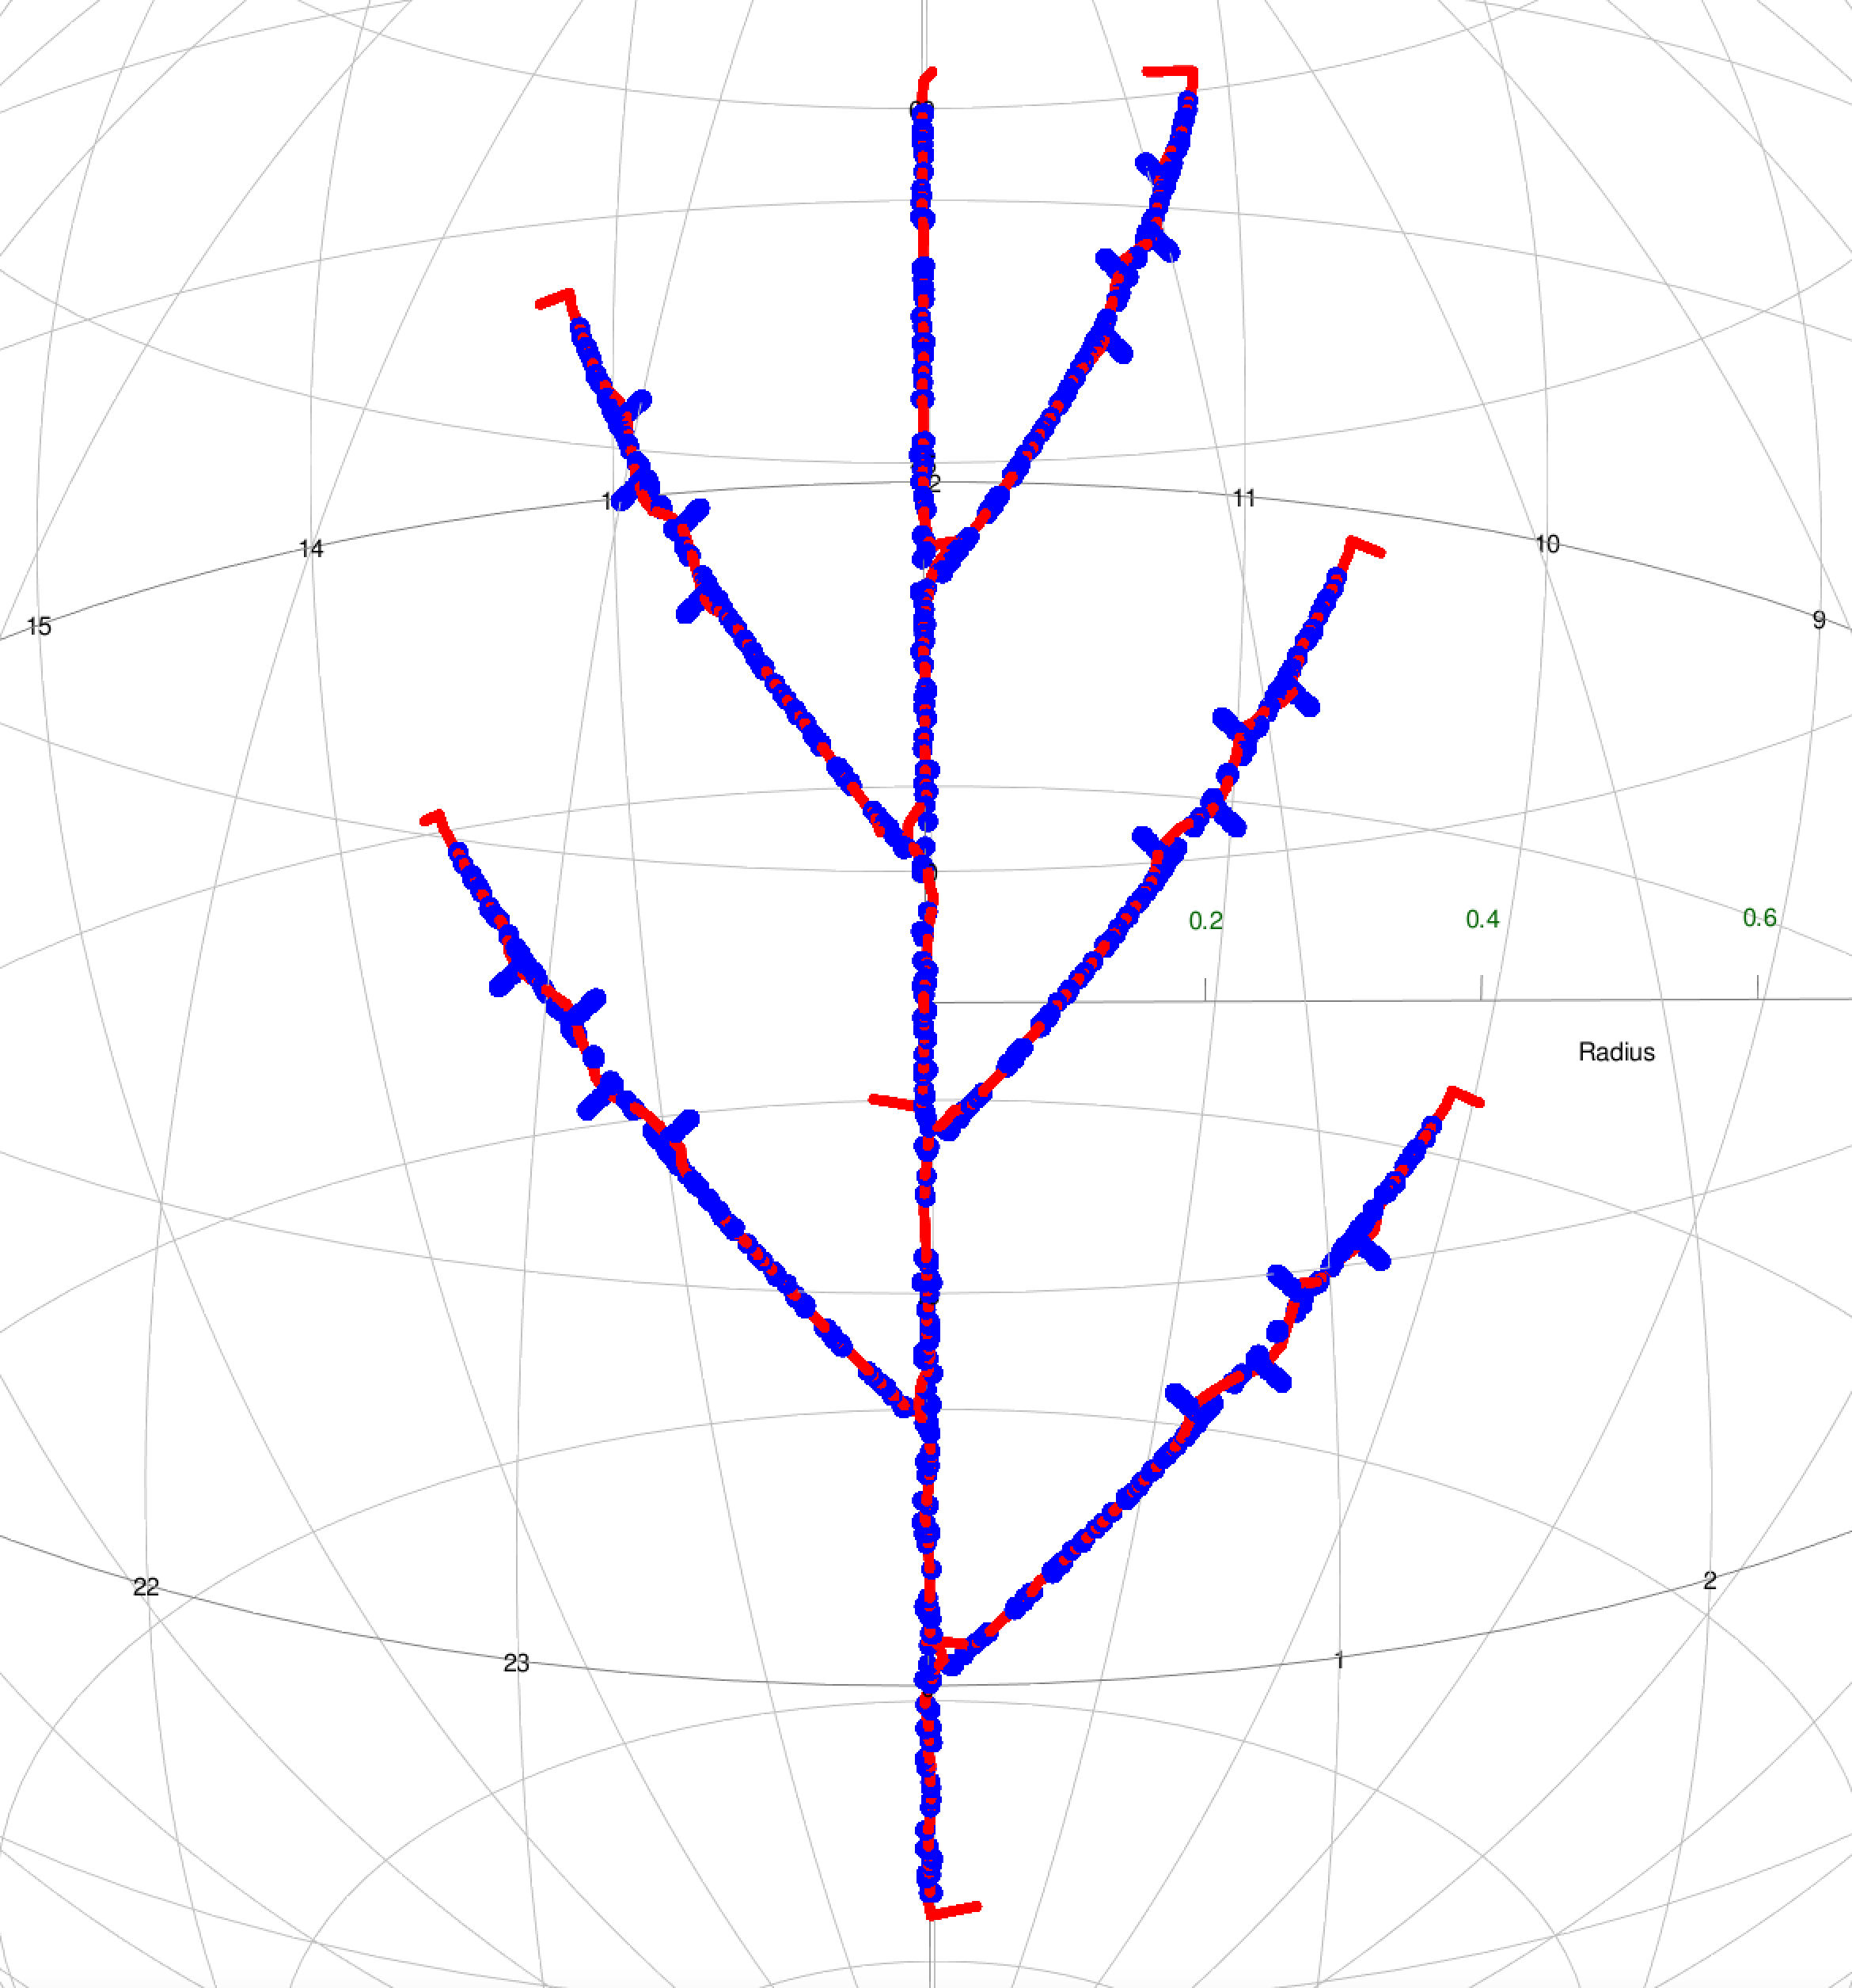
\includegraphics[scale=0.12]{figures/LPG(tree).png}
    \caption{Tree data (blue) and the result (red) of LPG with $\mbox{scale}=0.03$ and \text{nu}=0.2. The LPG function captures the complex structures of the data well, provided that \text{scale} and \text{nu} are properly chosen.}
    \label{fig:tree}
\end{figure}

As displayed in Figures~\ref{fig:spiral}, \ref{fig:zigzag}, and \ref{fig:tree}, the \code{LPG()} function identifies the non-geodesic or complex patterns of the simulated datasets well as long as the parameters of $\mbox{scale}~\mbox{and}~\mbox{nu}$ are properly chosen. The arguments and outputs of the function are respectively described in Tables~\ref{table:LPG} and \ref{table:LPGout}.

\begin{table}[!ht]
\centering
\begin{tabular}{lp{0.82 \textwidth}}
\toprule
Argument & Description \\
\midrule	
\code{data} & matrix or data frame consisting of spatial locations with two columns. Each row represents longitude and latitude (denoted by degrees). \\
\code{scale} & scale parameter for this function. The argument is the degree to which the \code{LPG} function expresses data locally; thus, as the \code{scale} grows, the result of the \code{LPG} becomes similar to that of the \code{PGA} function. The default is 0.4. \\
\code{tau} & forwarding or backwarding distance of each step. It is empirically recommended to choose a third of \code{scale}, which is the default of this argument. \\
\code{nu} & parameter to alleviate bias of resulting curves. \code{nu} represents the viscosity of the given data and it should be selected in $[0,\, 1)$. The default is zero. When \code{nu} is close to 1, the curve usually swirls similarly to the motion of a large viscous fluid. The argument \code{maxpt} can control the swirling. \\
\code{maxpt} & maximum number of points in each curve. The default is 500. \\
\code{seed} & random seed number. \\
\code{kernel} & kind of kernel function. The default is the indicator kernel, and the alternative is quartic or Gaussian. \\
\code{thres} & threshold of the stopping condition for the \code{IntrinsicMean} function in the process of the \code{LPG} function. The default is 1e-4. \\
\code{col1} & color of data. The default is blue. \\ 
\code{col2} & color of points in the resulting principal curves. The default is green.\\
\code{col3} & color of the resulting curves. The default is red.\\
\bottomrule
\end{tabular}
\caption{Arguments of the \code{LPG()}.}
\label{table:LPG}
\end{table}

\begin{table}[!ht]
\centering
\begin{tabular}{lp{0.82 \textwidth}}
\toprule
Output & Description \\
\midrule
\code{plot} & plotting of the result in 3D graphics. \\
\code{num.curves} & the number of resulting curves. \\
\code{prin.curves} & spatial locations (represented by degrees) of points in the resulting curves. \\ 
\code{line} & connecting lines between points in \code{prin.curves}. \\
\bottomrule
\end{tabular}
\caption{Outputs of the \code{LPG()}.}
\label{table:LPGout}
\end{table}

\section{Application}
\begin{figure}[h]
    \centering
    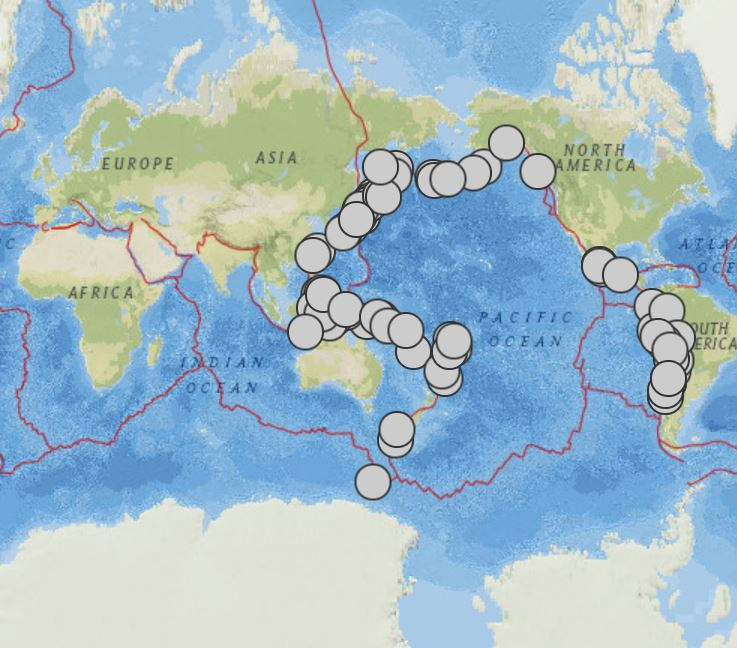
\includegraphics[scale=0.46]{{figures/earthquake1.png}}
    \hspace{0.4cm}
    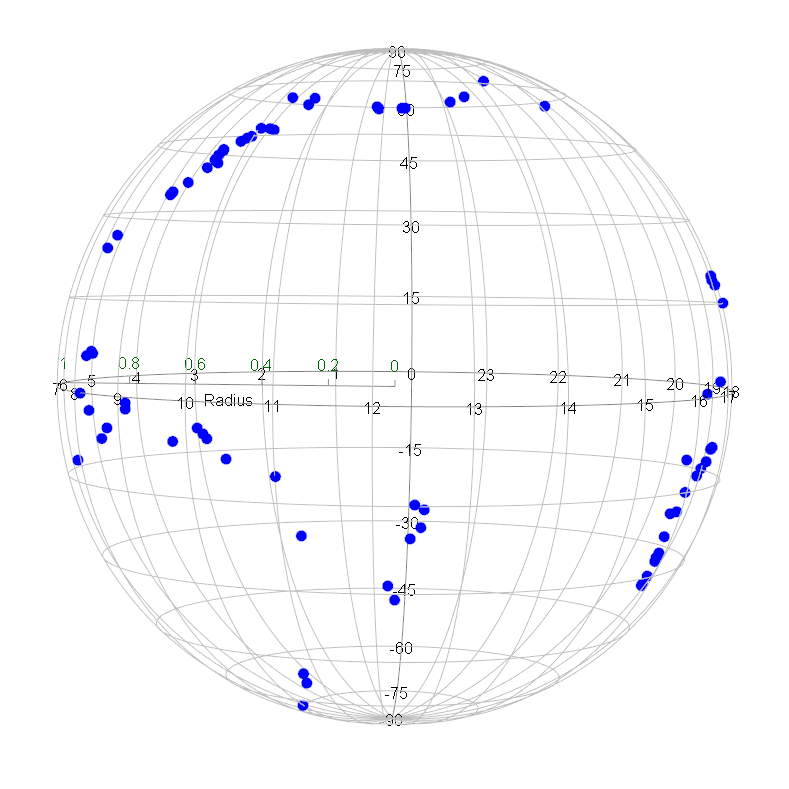
\includegraphics[scale=0.28]{{figures/earthquake2.png}}
    \caption{The distribution of significant earthquakes (8+ Mb magnitude), and their three-dimensional visualization.}
    \label{fig:earthquake}
\end{figure}
We use earthquake data from the U.S. Geological Survey, which has collected significant earthquakes (8+ Mb magnitude) around the Pacific Ocean since 1900. As shown in Figure~\ref{fig:earthquake}, the data contain 77 observations distributed in the borders between the Eurasian, Pacific, North American, and Nazca tectonic plates. The data have three features: the observations are distributed globally, scattered, and form non-geodesic structures. Because the tectonic plates are constantly moving in different directions, identifying the hidden patterns of borders is useful in geostatistics and seismology, as noted in \cite{Biau, Mardia2014}. It can be possible to identify the borders of plates by applying dimension reduction methods to the earthquake data. 

To apply the aforementioned dimension reduction methods to the earthquake data, we use the following code. %The corresponding results are shown in Figures~ \ref{fig:PGAPC}, \ref{fig:SPC}, \ref{fig:SPC:change}, and \ref{fig:LPG}, respectively.
\begin{example}
   > data(Earthquake)
   #### collect spatial locations (longitude and latitude by degrees) of data
   > earthquake <- cbind(Earthquake$longitude, Earthquake$latitude)  

   #### example 1: principal geodesic analysis (PGA)
   > PGA(earthquake)

   #### example 2: principal circle
   ## get center and radius of principal circle
   > circle <- PrincipalCircle(earthquake)    
   ## generate the principal circle
   > PC <- GenerateCircle(circle[1:2], circle[3], T = 1000)   
   ## plot the principal circle
   > sphereplot::rgl.sphgrid(col.long = "black", col.lat = "black")                                  
   > sphereplot::rgl.sphpoints(earthquake, radius = 1, col = "blue", size = 12)
   > sphereplot::rgl.sphpoints(PC, radius = 1, col = "red", size = 9)
\end{example}
Examples 1 and 2 implement the principal geodesic and the principal circle, respectively. As illustrated in Figure~\ref{fig:PGAPC}, the principal geodesic (left) fails to identify the variations of the earthquake data. The principal circle (right) captures the global trend of the data, whereas the circle could not extract the local variations of the data.

\begin{figure}[h]
    \centering
    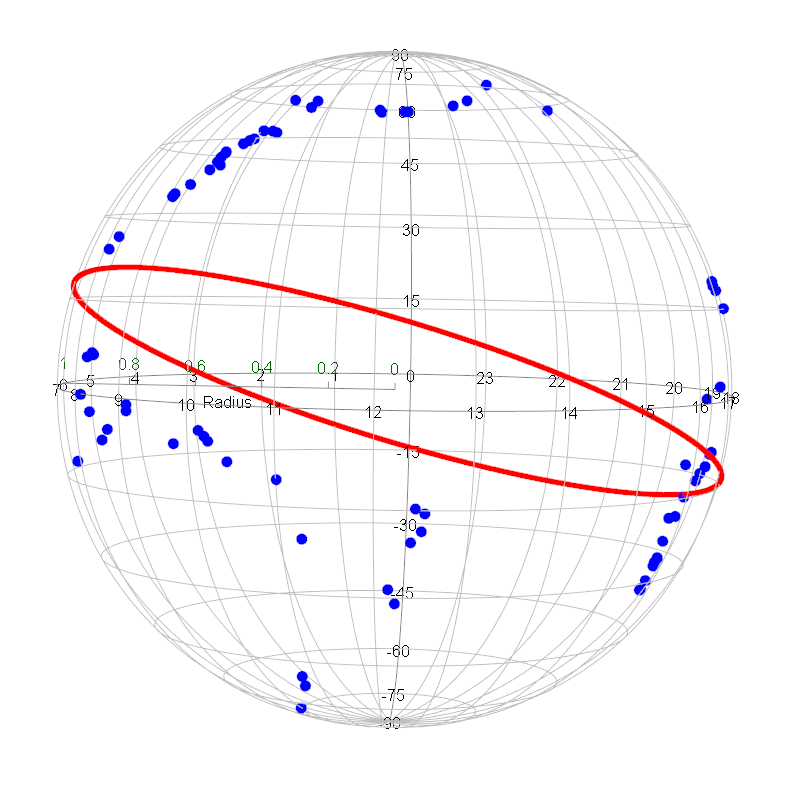
\includegraphics[scale=0.265]{figures/PGA(earthquake).png}
    \hspace{1cm}
    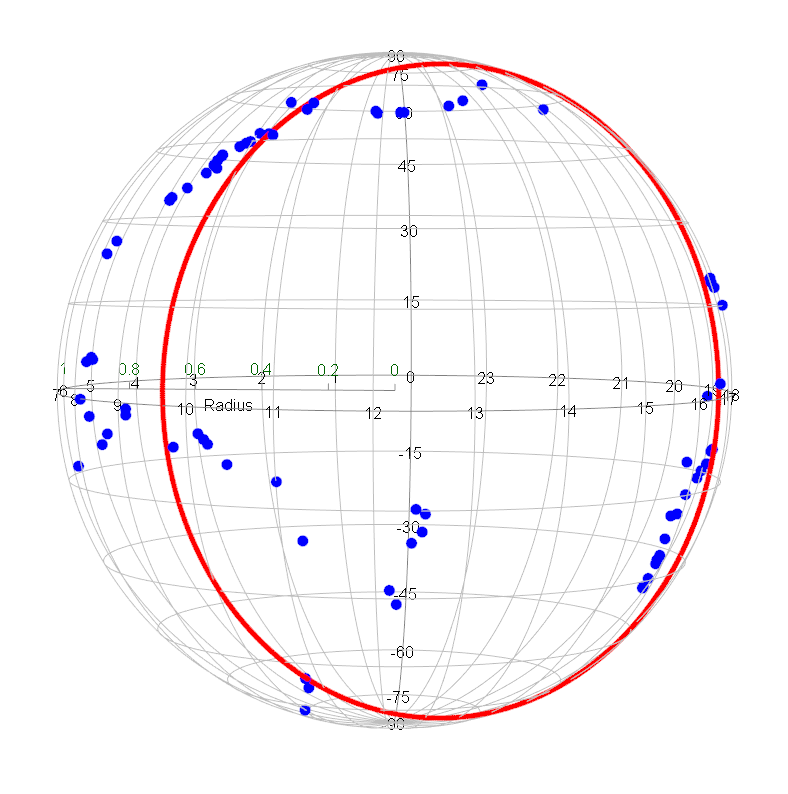
\includegraphics[scale=0.265]{figures/PC(earthquake).png}
    \caption{Earthquake data (blue) and the results (red) of the principal geodesic analysis and principal circle, from left to right. The principal geodesic fails to find the non-geodesic feature of the data, and the principal circle captures the circular pattern but cannot identify the local variations of the data.} 
    \label{fig:PGAPC}
\end{figure}

\begin{figure}[!h]
    \centering
    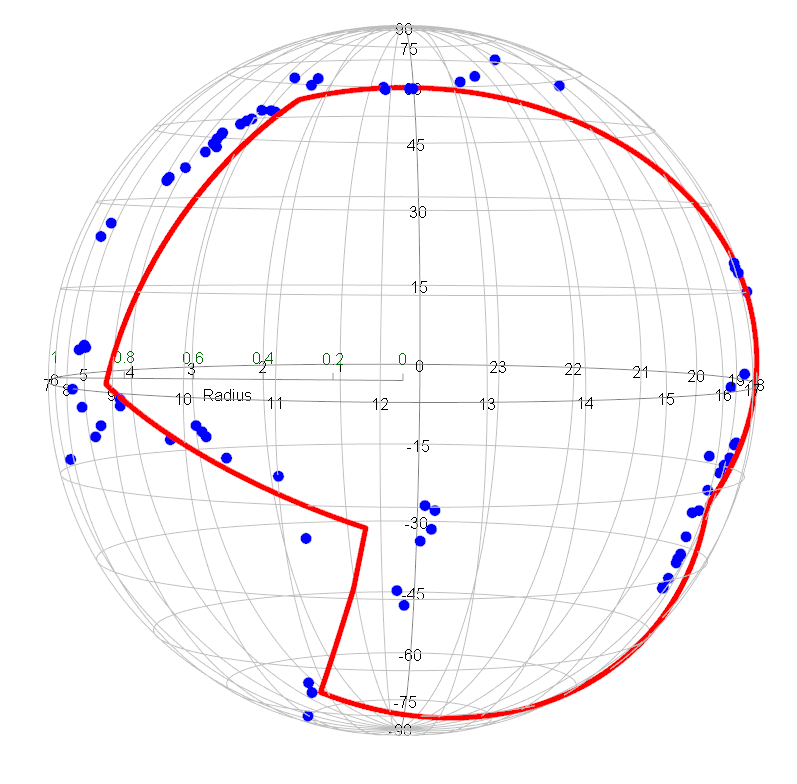
\includegraphics[scale=0.265]{figures/SPCHauberg(earthquake).png}
    \hspace{0.6cm}
    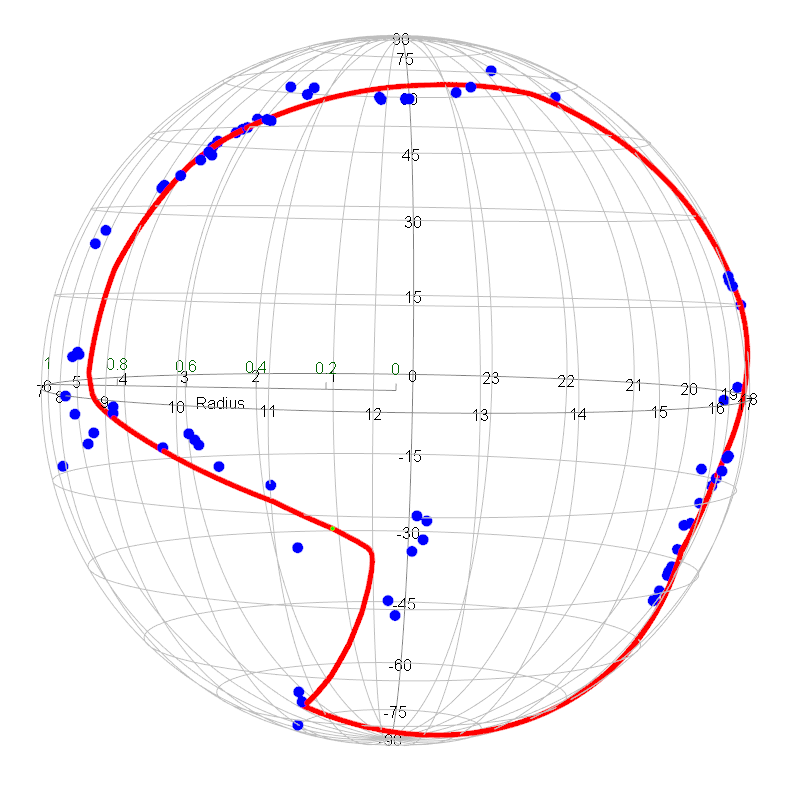
\includegraphics[scale=0.265]{figures/SPC(earthquake).png}
    \caption{Earthquake data (blue) and implementation results (red) with $q = 0.1$ of the SPC.Hauberg and SPC functions, respectively, from left to right. Both methods can represent the non-geodesic feature of the earthquake data. The spherical principal curve particularly tends to be smoother.} 
     \label{fig:SPC}
\end{figure}

\begin{example}
   #### example 3: spherical principal curves and principal curves of Hauberg
   > SPC.Hauberg(earthquake, q = 0.1) # principal curves of Hauberg
   > SPC(earthquake, q = 0.1)         # spherical principal curves
\end{example}
Example 3 fits the spherical principal curve and Hauberg's principal curve with $q=0.1$. As shown in Figure~\ref{fig:SPC}, both methods identify the curved feature of the earthquake data. The spherical principal curve particularly tends to be more continuous than Hauberg's principal curve.

\begin{example}
   #### example 4: spherical principal curves with q = 0.15, 0.1, 0.03, and 0.02
   > SPC(earthquake, q = 0.15)         
   > SPC(earthquake, q = 0.1)
   > SPC(earthquake, q = 0.03)
   > SPC(earthquake, q = 0.02)
\end{example}
Example 4 applies the spherical principal curve to the earthquake data with varying $q=0.15,\, 0.1,\, 0.03,\, 0.02$. The parameter $q$ plays a role in the bandwidth of the \code{SPC()} function. As shown in Figure~\ref{fig:SPC:change}, the smaller $q$ is, the rougher the curve is. On the contrary, the larger $q$ is, the smoother the curve is.

\begin{figure}[h]
    \centering
    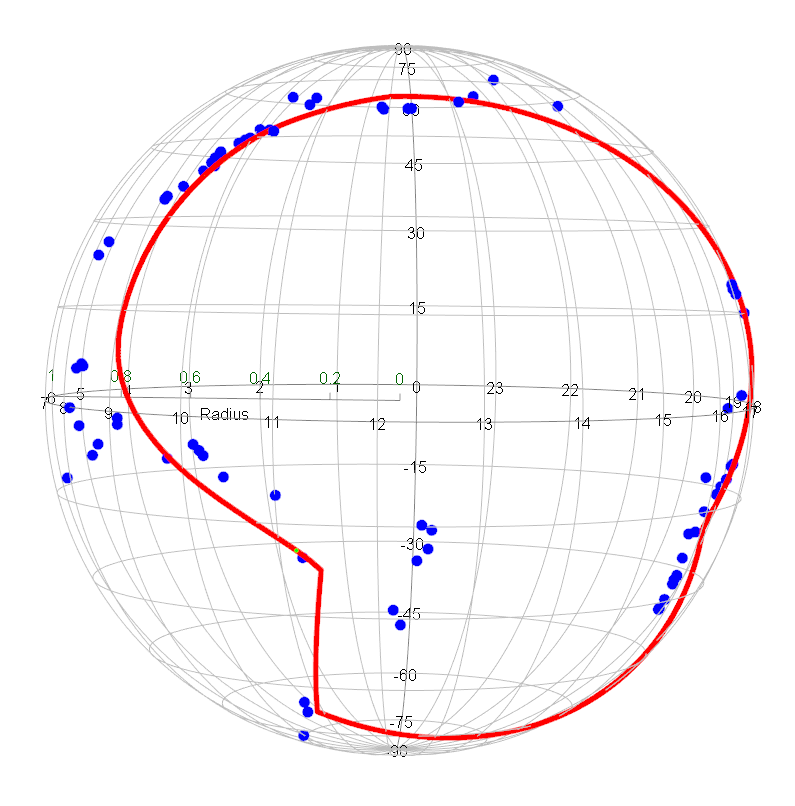
\includegraphics[scale=0.255]{figures/SPC(earthquake)q=015.png}
    \hspace{0.8cm}
    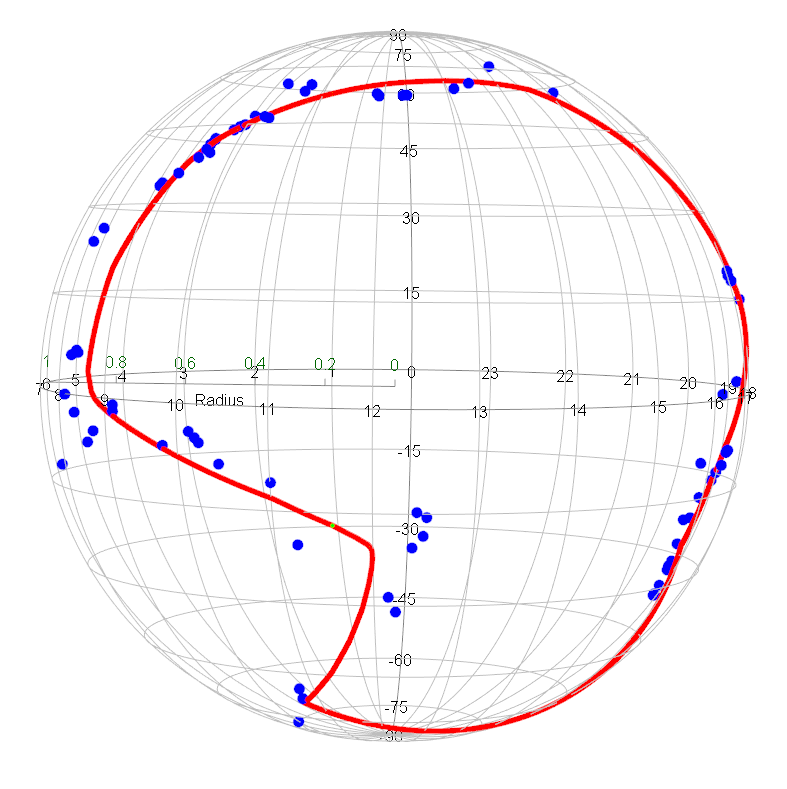
\includegraphics[scale=0.255]{figures/SPC(earthquake)q=01.png}
    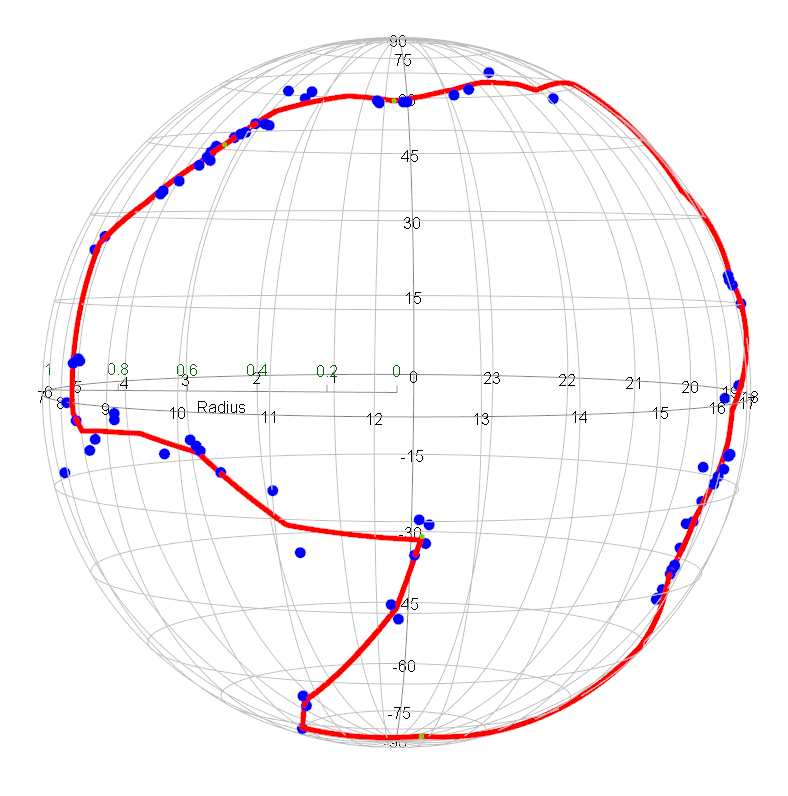
\includegraphics[scale=0.25]{figures/SPC(earthquake)q=003.png}
    \hspace{0.8cm}
    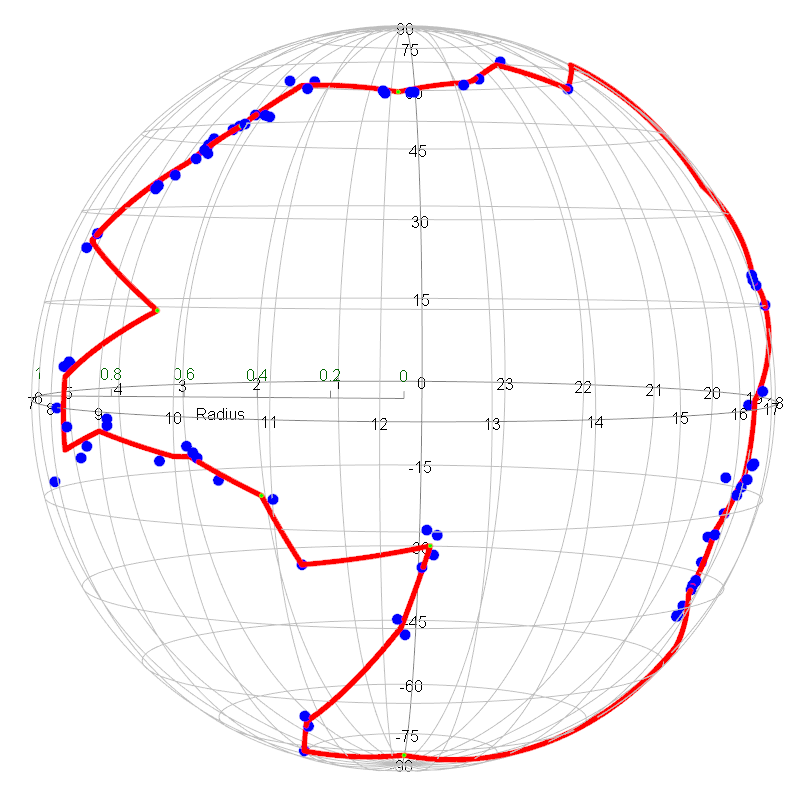
\includegraphics[scale=0.24]{figures/SPC(earthquake)q=002.png}
    \vspace{0cm}
    \caption{From left to right and top to bottom: Earthquake data (blue) and the results (red) of the SPC with $q=0.15,~ 0.1,~ 0.03~ \mbox{and}~ 0.02$. The larger the parameter $q$ is, the smoother the curve is, while it tends to underfit the data. Conversely, the smaller the parameter $q$ is, the rougher the curve is.}
    \label{fig:SPC:change}
\end{figure}

\begin{example}
   #### example 5: local principal geodesics (LPG)
   > LPG(earthquake, scale = 0.5, nu = 0.2, maxpt = 20, seed = 50)
   > LPG(earthquake, scale = 0.4, nu = 0.3, maxpt = 22, seed = 50)  
\end{example}
Lastly, example 5 implements the \code{LPG()} function with different \code{scale} and \code{nu}. As shown in Figure~\ref{fig:LPG}, the function represents the curved pattern of the data, illustrating the slightly different features.

\begin{figure}[!h]
    \centering
    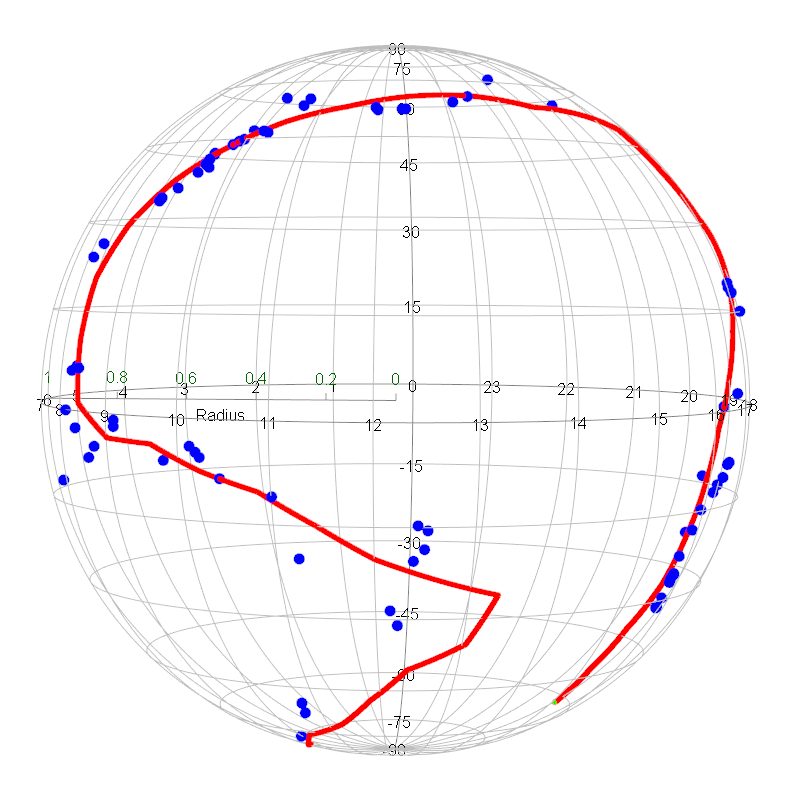
\includegraphics[scale=0.25]{figures/LPG(earthquake).png}
    \hspace{1cm}
    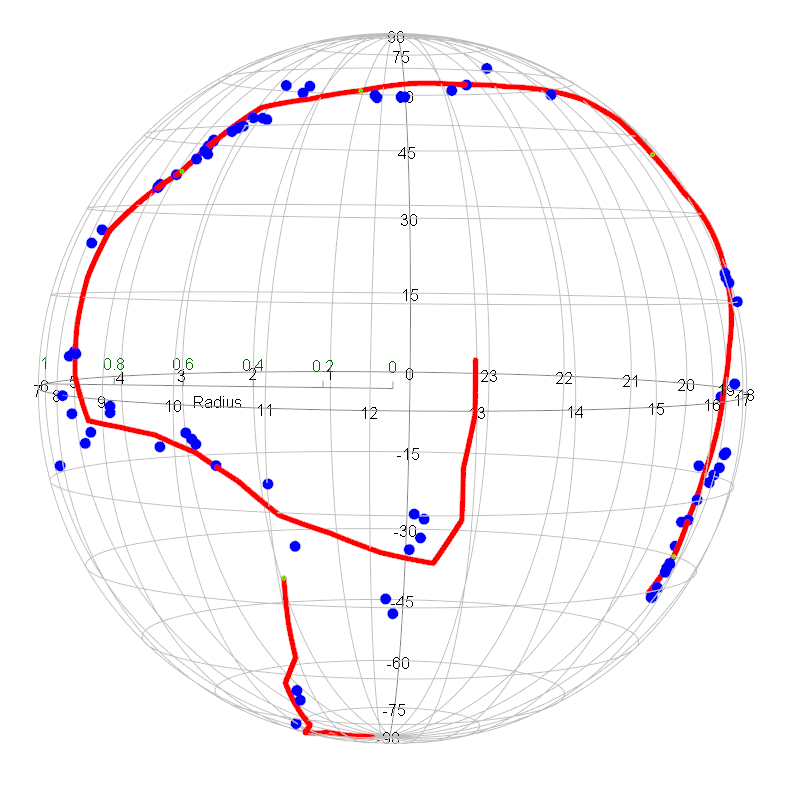
\includegraphics[scale=0.25]{figures/LPG(earthquake)2.png}
    \caption{From left to right, earthquake data (blue) and the results of the LPG function with $\mbox{scale}=0.5$, nu=0.2 and $\mbox{scale}=0.4$, nu=0.3. Both the local principal geodesics implemented by different parameters recognize the non-geodesic and scattered pattern of the data, illustrating the different features.}
    \label{fig:LPG}
\end{figure}

\section{Conclusions}
In this paper, the R package \CRANpkg{spherepc} has implemented various dimension reduction methods on a sphere. It includes not only principal geodesic analysis (PGA), principal circle, and principal curves of \citet{Hauberg2016} as existing methods but also spherical principal curves (SPC) and local principal geodesics (LPG) as new approaches. The \CRANpkg{spherepc} package has demonstrated its usefulness by applying the functions to several simulation examples and real earthquake data. We believe that the \CRANpkg{spherepc} is helpful for applications in various fields, ranging from statistics to engineering, such as geostatistics, image analysis, pattern recognition, and machine learning.

\section{Acknowledgments}
This research was supported by the National Research Foundation of Korea (NRF) funded by the Korea government (2020R1A4A1018207; 2021R1A2C1091357).

\bibliography{RJspherepc}


%\bibliography{Lee-Kim-Oh}

\address{Jongmin Lee\\
  Department of Statistics\\
  Seoul National University\\
  Seoul 08826, Korea\\
  (ORCiD 0000-0003-1723-4615)\\
  \email{jongminlee9218@gmail.com}}

\address{Jang-Hyun Kim\\
  Department of Computer Science and Engineering\\
  Seoul National University\\
  Seoul 08826, Korea\\
  (ORCiD 0000-0001-8433-2712)\\
  \email{kimjanghyun1230@gmail.com}}
  
\address{Hee-Seok Oh\\
  Department of Statistics\\
  Seoul National University\\
  Seoul 08826, Korea\\
  (ORCiD 0000-0002-1501-0530)\\
  \email{heeseok@stats.snu.ac.kr}}
 
%\end{document}


\end{article}

\end{document}
